\chapter{Deep Learning Networks}
\section{Introduction}
Deep learning is a multidisciplinary field ranging from linear algebra, calculus and probability theory. With major advancement made in compute processing power; deep learning is commonly used in the industry now.
\vspace{5mm}
\\
\noindent\textbf{McCullough and Walter Pitts (MCP) Neuron}\\
In 1943, McCulloch and Walter Pitts demonstrated that simple binary threshold units wired up as logical gates could be used to build a digital computer (add-ref). The McCulloch-Pitts (MCP) neuron is a simple mathematical model of a biological neuron. It was the earliest mathematical model of a neural network and had only three types of weights; excitatory (1), inhibitory (-1) and inactive (0). The model had an activation function which had a value of 1 if the weighted sum was greater or equal to a given threshold, else 0. Using the MCP neuron, one of the first digital computers that contained stored programs was built. However, the MCP neuron was very restrictive.
\vspace{5mm}
\\
\noindent\textbf{Rosenblatt’s Perceptron Algorithm}\\
In 1958, Frank Rosenblatt proposed the perceptron and an algorithm to adjust weights of the MCP neuron, extending the work done by McCulloch and Pitts. The MCP neuron had some limitations that the Perceptron managed to solve, for example the input was not restricted to boolean values but expanded to real numbers. Rosenblatt proved that if the data used to train the perceptron are linearly separable classes, then the perceptron algorithm convergences and separates the two classes by a hyperplane.
\vspace{5mm}
\section{Perceptron}
\begin{figure}[ht]
  \centering
  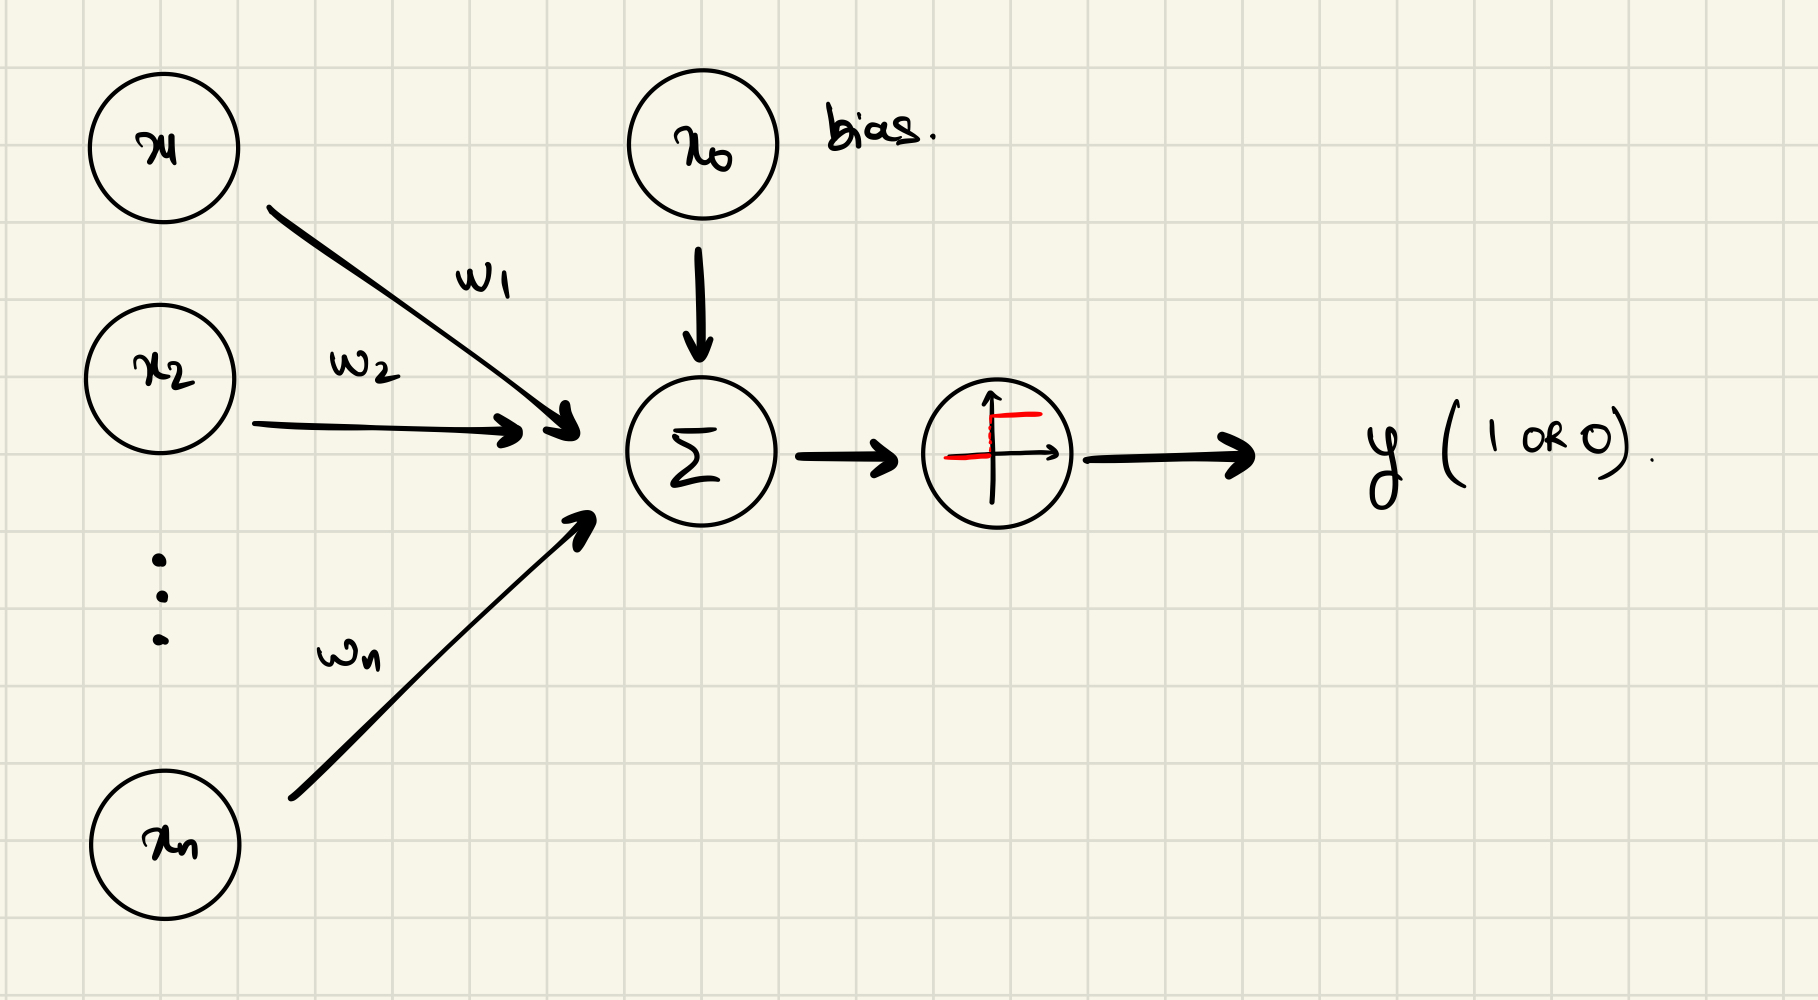
\includegraphics[scale=0.15]{CHAPTER_2/c2_fig_perceptron_2.jpeg}
  \caption{Rosenblatt perceptron}
  \label{rosenblatt_perceptron}
\end{figure}
\vspace{5mm}
\noindent Let $\textbf{x}$ be a vector of inputs where each $x_i \in \mathbb{Z}$ and $\textbf{w}$ be a vector of weights corresponding to the input signals where each $w_i \in \mathbb{Z}$. 
\begin{align}
  \begin{matrix}
    \textbf{x} = \begin{bmatrix}
      x_{0} \\
      x_{1} \\
      \vdots \\
      x_{n}
    \end{bmatrix}, & \textbf{w} = \begin{bmatrix}
      w_{0} \\
      w_{1} \\
      \vdots \\
      w_{n}
    \end{bmatrix}
  \end{matrix} \nonumber
\end{align}
\noindent Then, the mathematical definition of the perceptron is given by
\begin{align}
  \phi(z) = \begin{cases}
    1 & \text{if } \sum^{n}_{i=0} w_ix_i \geq  0\\
    0 & \text{otherwise}
    \label{eq:mcp_neuron}
  \end{cases}
\end{align}
\vspace{5mm}
\\
where $\phi(z)$ is known as the hard delimiter.
\vspace{5mm}
\\
\noindent Consider the two sets of point \textbf{A} and \textbf{B} 
\begin{align}
  \textbf{A} =
  \begin{Bmatrix}
    \begin{bmatrix}
      1 \\ 
      2
    \end{bmatrix}
  \end{Bmatrix}
   \, \, \, 
  \textbf{B} =
\begin{Bmatrix}
  \begin{bmatrix}
    -1 \\
    2
  \end{bmatrix},
  \begin{bmatrix}
    0 \\
    -1
  \end{bmatrix}
  \end{Bmatrix}
\end{align}
and fitting the perceptron function (\refeq{eq:mcp_neuron}) to learn how to classify points in each respective set. Let set \textbf{A} and \textbf{B} be class 1 and 0 respectively.
\begin{figure}[ht]
  \centering
  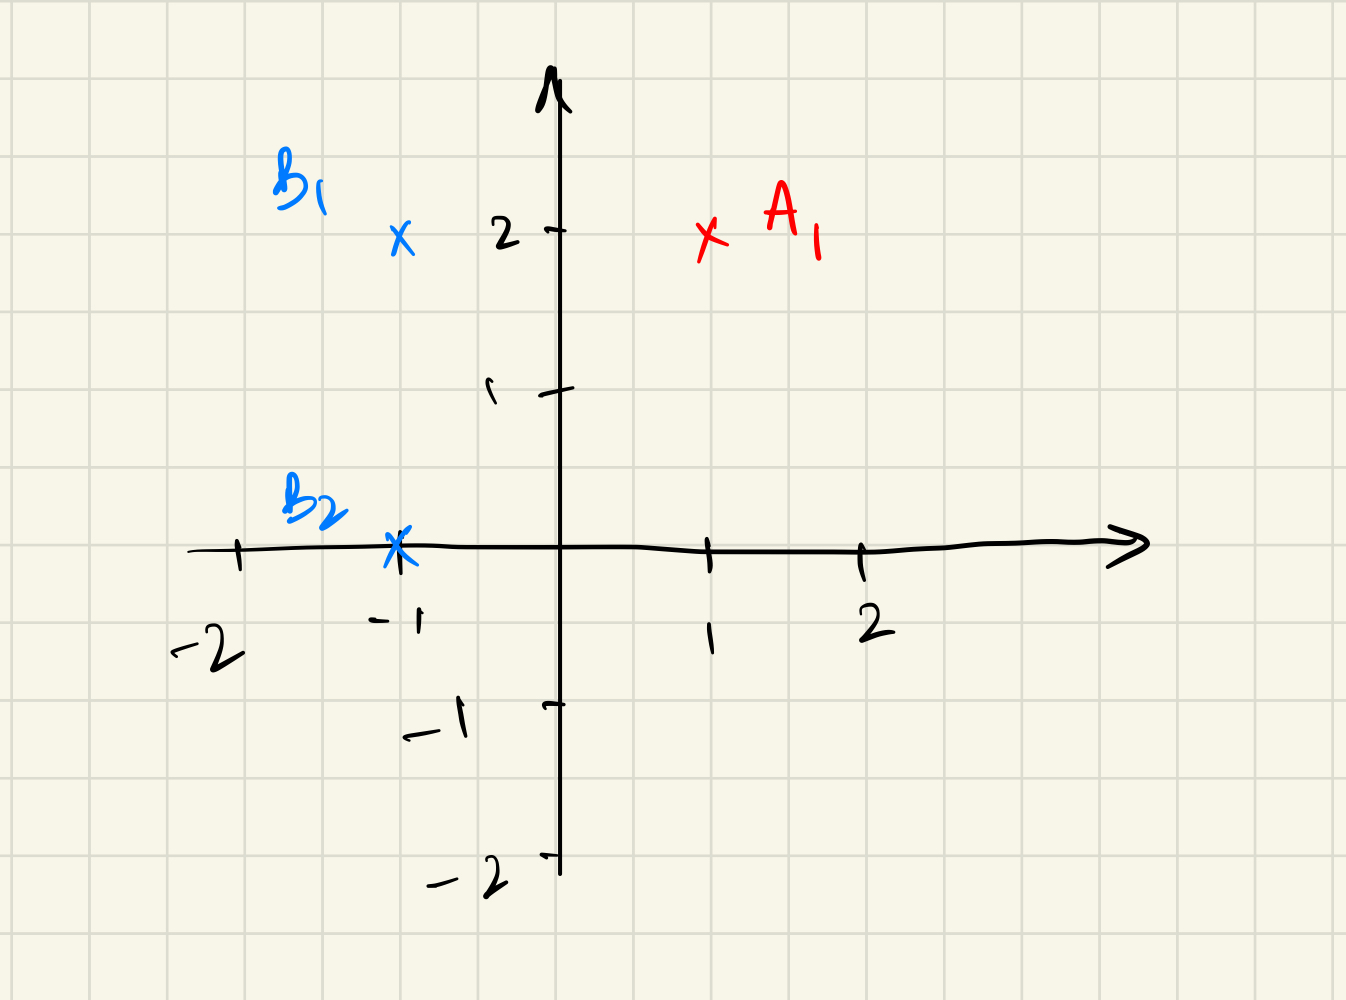
\includegraphics[scale=0.15]{CHAPTER_2/c2_fig_perceptron_example_1.jpeg}
  \caption{Caption}
  \label{fig:perceptron_example_1}
\end{figure}\\
From \ref{fig:perceptron_example_1}, we can separate the two classes by a single line. Consider the random separating line passing through the origin (this will set the value of $x_0$ in (\refeq{eq:mcp_neuron}) to 0).\\
\begin{figure}[!htbp]
  \centering
  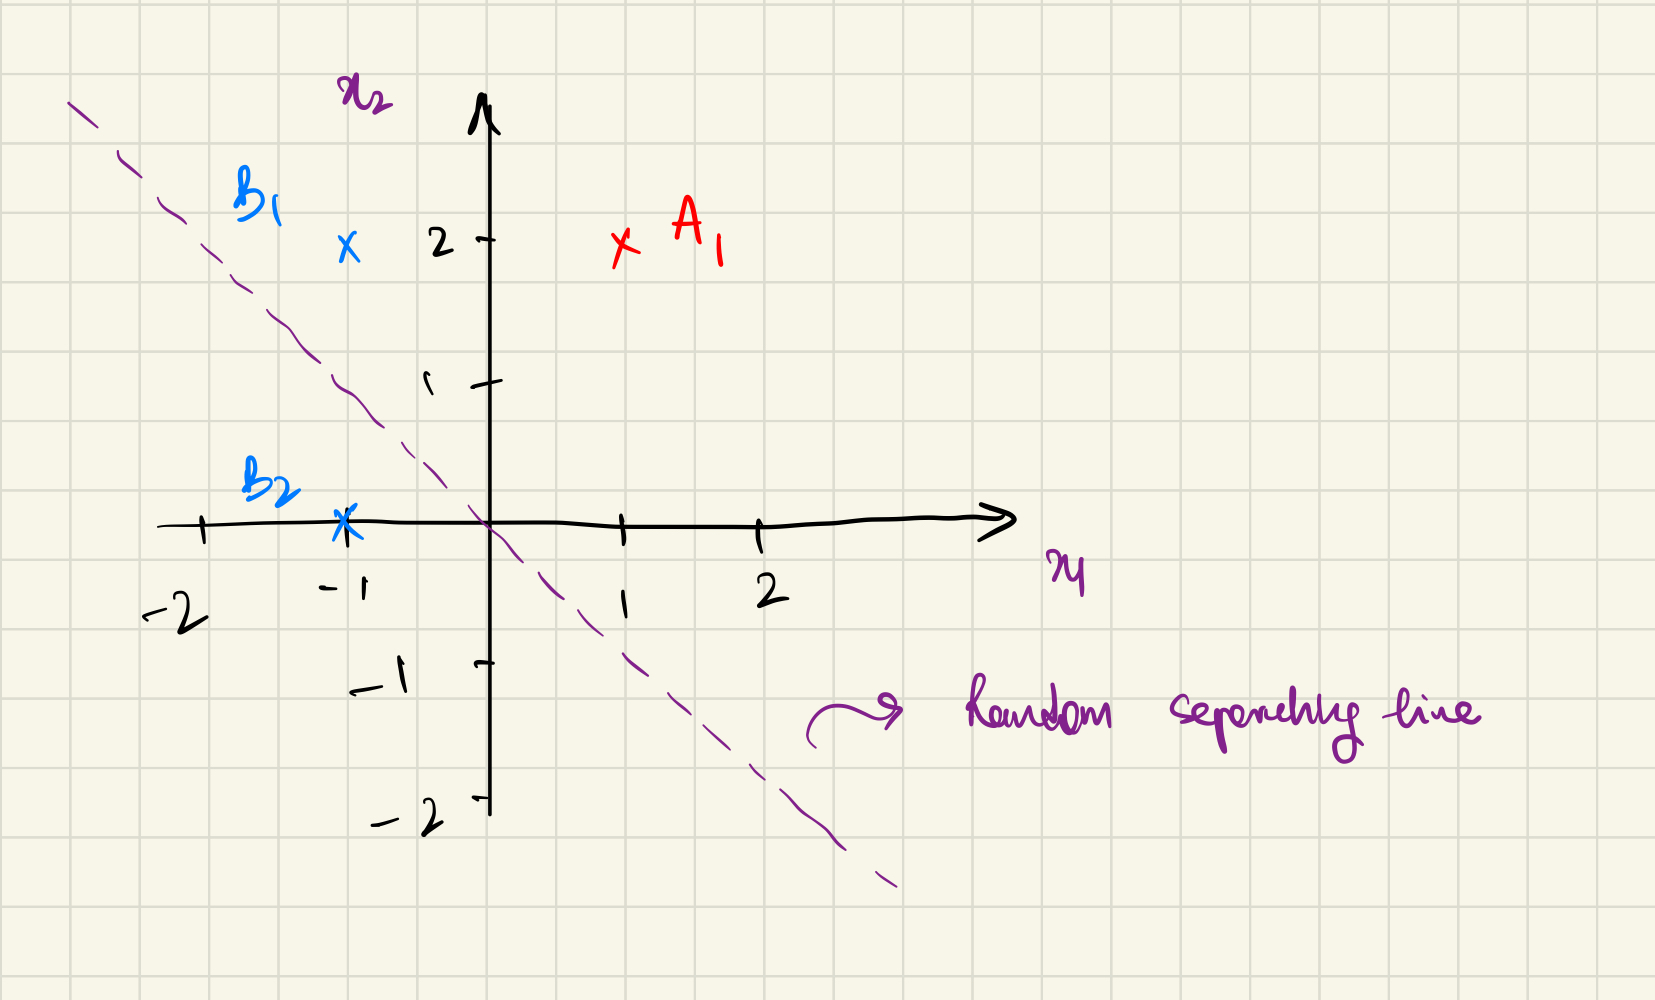
\includegraphics[scale=0.15]{CHAPTER_2/c2_fig_perceptron_example_2.jpeg}
  \caption{Caption}
  \label{fig:perceptron_example_2}
\end{figure}\\
The equation of the random line is given by
\begin{align}
  x_1 = - x_2
\end{align}
Comparing to the equation (\refeq{eq:mcp_neuron}); we can deduce that 
\begin{align}
  \begin{matrix}
    w_1 = 1 & w_2 = 1
  \end{matrix}
\end{align}
Visually, we can already see that the separating line does not split the points properly. The computation of the binary classification using the random line is given by
\begin{align}
  \phi(A_1) &= \phi\begin{pmatrix}
    \begin{bmatrix}
      1\\
      1
    \end{bmatrix}.\begin{bmatrix}
      1 \\
      2
    \end{bmatrix}
  \end{pmatrix} = \phi(3) = 1 \\
  \phi(B_1) &= f\begin{pmatrix}
    \begin{bmatrix}
      1\\
      1
    \end{bmatrix}.\begin{bmatrix}
      -1 \\
      2
    \end{bmatrix}
  \end{pmatrix} = \phi(1) = 1 \\
  \phi(B_2) &= f\begin{pmatrix}
    \begin{bmatrix}
      1\\
      1
    \end{bmatrix}.\begin{bmatrix}
      -1 \\
      0
    \end{bmatrix}
  \end{pmatrix} = \phi(-1) = 0
\end{align}
The computation confirms the visual representation and groups $\textbf{A}_1$ and $\textbf{B}_1$ together and $\textbf{B}_2$ separated which is incorrect. We can either alter the separating line (by moving the weight vector) with respect to $\textbf{A}_1$ and/or $\textbf{B}_1$.
\begin{figure}[ht]
  \centering
  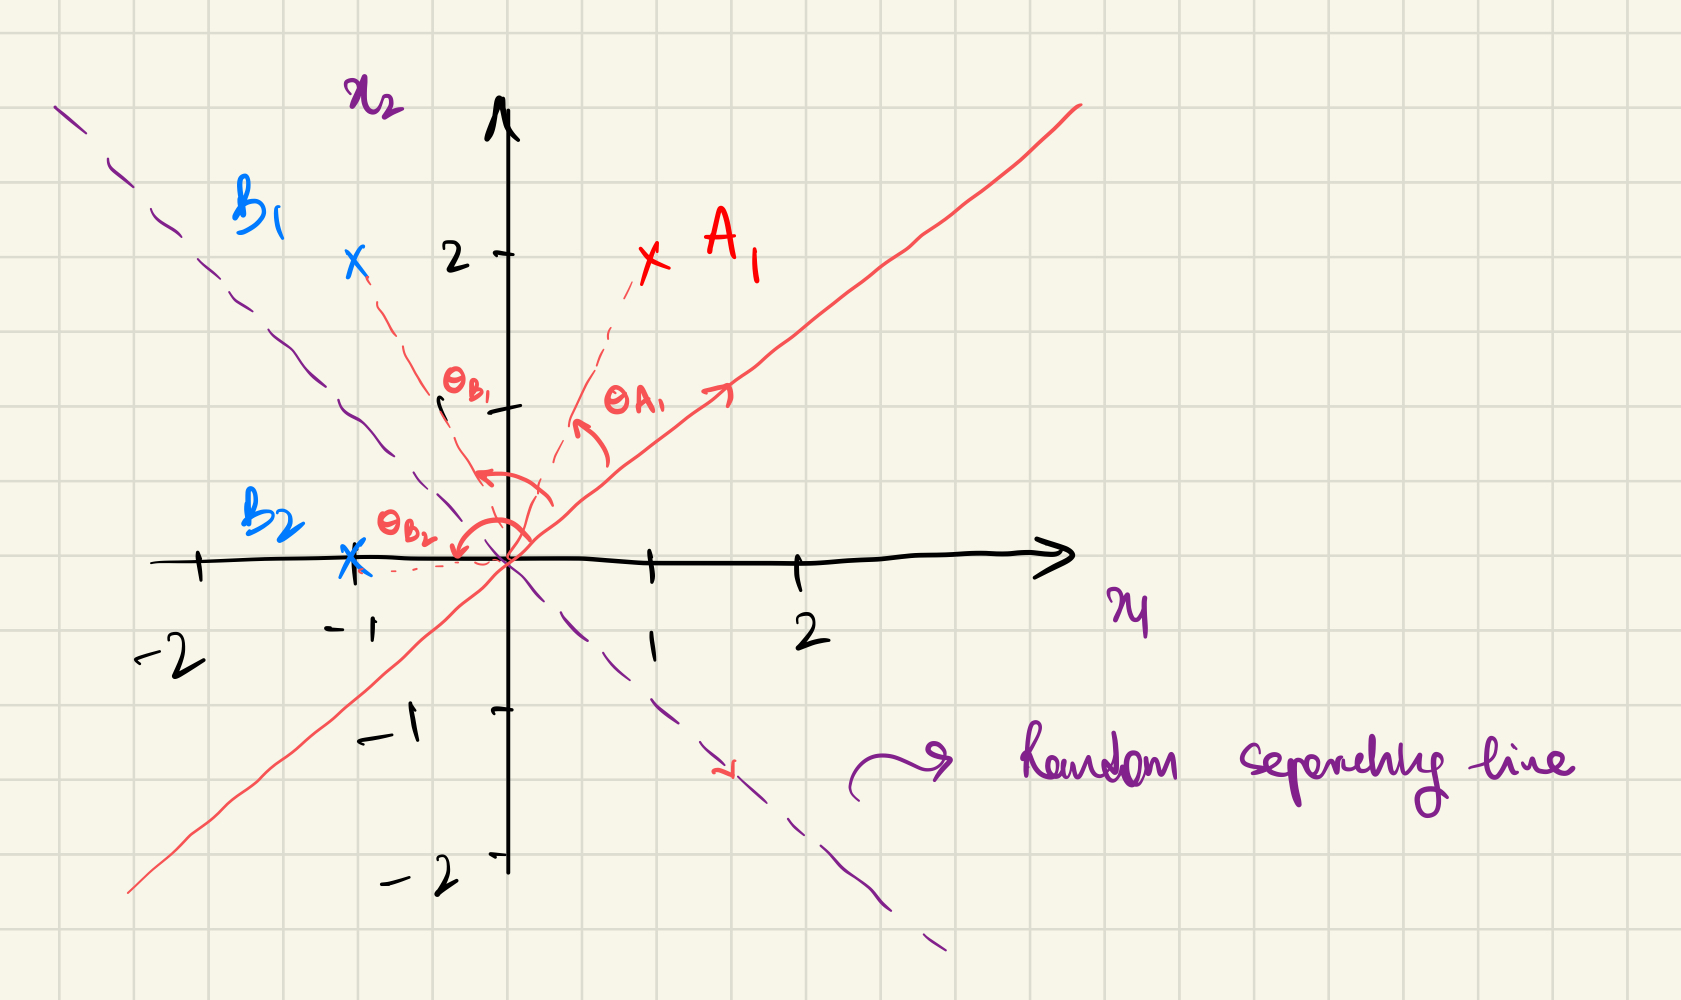
\includegraphics[scale=0.25]{CHAPTER_2/c2_fig_perceptron_example_3.jpeg}
  \caption{!!!TO BE CHANGED!!!}
  \label{fig:perceptron_example_3}
\end{figure}\\
Since $\textbf{B}_1$ is incorrectly classified, using the property of subtraction of vectors; we move the weight vector ($\textbf{w}$) away from $\textbf{B}_1$ and check the classification again.
\begin{align}
  \textbf{w}^{(1)} &= \textbf{w} - \textbf{B}_1 \\
  &= \begin{bmatrix}
    1 \\
    1
  \end{bmatrix} - \begin{bmatrix}
    -1 \\
    2
  \end{bmatrix} \\
  & = \begin{bmatrix}
    2 \\
    -1
  \end{bmatrix}
\end{align}\\
\begin{figure}[ht]
  \centering
  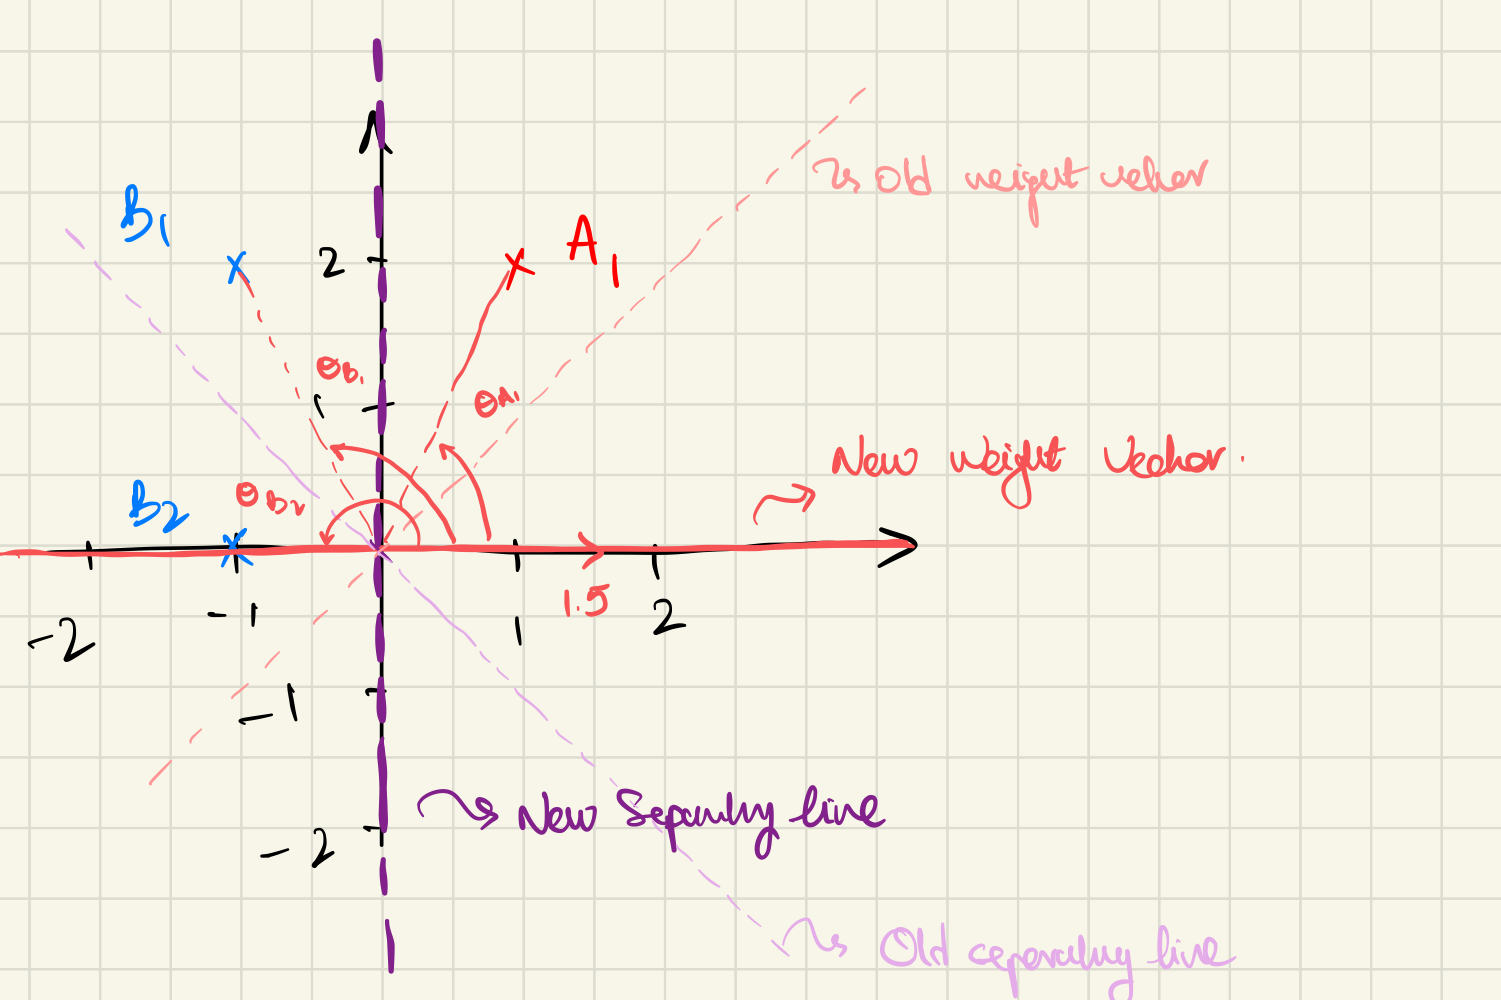
\includegraphics[scale=0.15]{CHAPTER_2/c2_fig_perceptron_example_4.jpeg}
  \caption{!!!!TO BE CHANGED!!!!}
  \label{fig:perceptron_example_4}
\end{figure} \\
Based on the new separating line, we can observe visually that the points are correctly classified. The computation of the binary classification using the new separating line $\textbf{w}^{(1)}$ is given by
\begin{align}
  \phi(A_1) &= \phi\begin{pmatrix}
    \begin{bmatrix}
      2\\
      -1
    \end{bmatrix}.\begin{bmatrix}
      1 \\
      2
    \end{bmatrix}
  \end{pmatrix} = \phi(0) = 1 \\
  \phi(B_1) &= \phi\begin{pmatrix}
    \begin{bmatrix}
      2\\
      -1
    \end{bmatrix}.\begin{bmatrix}
      -1 \\
      2
    \end{bmatrix}
  \end{pmatrix} = \phi(-4) = 0 \\
  \phi(B_2) &= \phi\begin{pmatrix}
    \begin{bmatrix}
      2\\
      -1
    \end{bmatrix}.\begin{bmatrix}
      -1 \\
      0
    \end{bmatrix}
  \end{pmatrix} = \phi(-2) = 0
\end{align}
Thus, the perceptron learned how to classify the two sets of points. The function $f(\textbf{x})$ could be re-used to classify new points added to the sets.
\vspace{5mm}
\\
\noindent\textbf{Perceptron Algorithm}\\
The perceptron algorithm adjusts the weights and as a result, the hard delimiter as well in order to linearly separate a set of binary labelled input.

\begin{algorithm}
\caption{Perceptron Algorithm}\label{alg:perceptron_algorithm}
\begin{algorithmic}[1]
\Require \\
Let $t=0$ and $\textbf{w} = \begin{bmatrix}
  0 & 0 & \dots & 0
\end{bmatrix}^T$ \\
Consider the training set D $s.t$ $D = C_1 \cup C_2$  \\
$C_1$ $\leftarrow$ input with label 1 \\
$C_2$ $\leftarrow$ input with label 0\\
\textbf{Start}
\While{!convergence}
  \State Select a random input $\textbf{x}$
  \If{$\textbf{x}\in A$ and $\textbf{w}.\textbf{x}<0$}
  \State $\textbf{w} = \textbf{w} + \textbf{x}$
  \EndIf
  \If{$\textbf{x}\in B$ and $\textbf{w}.\textbf{x}\geq0$}
  \State $\textbf{w} = \textbf{w} - \textbf{x}$
  \EndIf
\EndWhile
\end{algorithmic}
\end{algorithm}
\noindent If the input data are binary and linearly separable; then algorithm (\ref{alg:perceptron_algorithm}) converges. The proof of convergence of the algorithm is known as the \textbf{perceptron convergence theorem}. \vspace{5mm}
\section{Perceptron Convergence Theorem}
\textbf{Theorem}\\
Consider algorithm (\ref{alg:perceptron_algorithm}) and let $D$ be a set of training vectors which are linearly separable. Let $\textbf{w}^{*}$ be the weight vectors which defines the separating line with $||\textbf{w}^{*}|| = 1$. Then the number of mistakes $m$ made by the perceptron algorithm satisfies 
\begin{align}
  \begin{matrix}
    m \leq \dfrac{1}{\gamma^2} & \text{where} & \gamma = \underset{\textbf{x}\in D}{\min} \dfrac{|{\textbf{w}^*}^T\textbf{x}|}{||\textbf{x}||_2}
  \end{matrix}
\end{align}
\textbf{Note}
\begin{enumerate}
  \item Since, $||\textbf{w}^{*}|| = 1 \implies \cos (\theta) = \dfrac{{\textbf{w}^*}^T\textbf{x}}{||\textbf{x}||_2}$
  \item If $||\textbf{x}||_2 = 1$, that is, we scale all the training examples to have unit norm (which has no effect their orientation), then $\gamma = \underset{\textbf{x}\in D}{\min} |{\textbf{w}^*}^T\textbf{x}|$ is the minimum distance from any example $\textbf{x} \in D$ to the separating line.
\end{enumerate}
\textbf{Proof}\\
We first prove the inequality given by 
\begin{align}
  (\textbf{w}^ {(t+1)})^T\textbf{w}^{*} \geq (\textbf{w}^ {(t)})^T\textbf{w}^{*} + \gamma
  \label{eq:per_cov_ine_1}
\end{align}
\indent \textbf{State 1} \\
In state 1, let us consider \textbf{x} being positive ($\textbf{x} \in C_1$) and incorrectly classified then
\begin{align}
  \nonumber
  (\textbf{w}^ {(t+1)})^T\textbf{w}^{*} = (\textbf{w}^ {(t)} + \textbf{x})^T\textbf{w}^{*} =   (\textbf{w}^ {(t)})^T\textbf{w}^{*} + \textbf{x}^T\textbf{w}^{*}
\end{align}
Assuming that all $||\textbf{x}||_2 = 1$ then $\textbf{x}^T\textbf{w}^{*} \geq \gamma$ since $\gamma$ is the minimum. 
\begin{align}
  \label{eq:per_cov_ine_2}
  (\textbf{w}^ {(t+1)})^T\textbf{w}^{*} \geq (\textbf{w}^ {(t)})^T\textbf{w}^{*} + \gamma
\end{align}
Thus, we have proved (\ref{eq:per_cov_ine_1})  under \textbf{State 1}.\\
\indent \textbf{State 2} \\
In state 2, let us consider \textbf{x} being negative ($\textbf{x} \in C_2$) and incorrectly classified then
\begin{align}
  \nonumber
  (\textbf{w}^ {(t+1)})^T\textbf{w}^{*} = (\textbf{w}^ {(t)} - \textbf{x})^T\textbf{w}^{*} =   (\textbf{w}^ {(t)})^T\textbf{w}^{*} - \textbf{x}^T\textbf{w}^{*}
\end{align}
Since $\textbf{x} \in C_2 \implies |{\textbf{w}^*}^T\textbf{x}| = - \textbf{x}^T\textbf{w}^* \geq 0$ and $|\textbf{x}^T\textbf{w}^{*}| \geq \gamma$
\begin{align}
  \nonumber
  (\textbf{w}^ {(t+1)})^T\textbf{w}^{*} &= (\textbf{w}^ {(t)})^T\textbf{w}^{*} + |{\textbf{w}^*}^T\textbf{x}| \\
  \label{eq:per_cov_ine_3}
  (\textbf{w}^ {(t+1)})^T\textbf{w}^{*} &\geq (\textbf{w}^ {(t)})^T\textbf{w}^{*} + \gamma
\end{align}
Thus, we have proved (\ref{eq:per_cov_ine_1})  under \textbf{State 2}.\\
From (\ref{eq:per_cov_ine_2}) and (\ref{eq:per_cov_ine_3}), we have shown that $\forall \textbf{x}\in D$ that inequality (\ref{eq:per_cov_ine_1}) holds.\\
Assume that the inequality (\ref{eq:per_cov_ine_1}) holds for an arbitrary integer value $m$ and $m-1$
\begin{align}
  \label{eq:induction_1}
  (\textbf{w}^ {(m)})^T\textbf{w}^{*} \geq (\textbf{w}^ {(m-1)})^T\textbf{w}^{*} + \gamma \\
  \label{eq:induction_2}
  (\textbf{w}^ {(m-1)})^T\textbf{w}^{*} \geq (\textbf{w}^ {(m-2)})^T\textbf{w}^{*} + \gamma 
\end{align}
Merging inequality (\ref{eq:induction_1}) and (\ref{eq:induction_2}) gives us
\begin{align}
  \label{eq:induction_3}
  (\textbf{w}^ {(m)})^T\textbf{w}^{*} \geq (\textbf{w}^ {(m-2)})^T\textbf{w}^{*} + 2\gamma
\end{align}
Hence, by induction, after $M$ mistakes, inequality (\ref{eq:induction_3}) becomes
\begin{align}
  \label{eq:induction_starts}
  (\textbf{w}^ {(m)})^T\textbf{w}^{*} \geq (\textbf{w}^ {(0)})^T\textbf{w}^{*} + m\gamma
\end{align}
Since $\textbf{w}^{(0)} = \mathbf{0}$ (the zero vector), we have
\begin{align}
  \label{eq:perp_cov_result1}
  (\textbf{w}^ {(m)})^T\textbf{w}^{*} \geq m\gamma
\end{align}
Next, we show that 
\begin{align}
  ||{\textbf{w}^{(t+1)}}||_{2}^{2} \leq ||{\textbf{w}^{(t)}}||_{2}^{2} + 1
  \label{eq:induction_proof_part2}
\end{align}
\indent \textbf{State 1} \\
Consider the same state 1 as before, thus we have
\begin{align}
  \begin{matrix}
    \label{eq:state1_conditions}
    (\textbf{w}^ {(t)})^T\textbf{x} \leq 0 & \text{and} & \textbf{w}^ {(t+1)} = \textbf{w}^{(t)} + \textbf{x}
  \end{matrix}
\end{align}
then
\begin{align}
  \nonumber
  ||\textbf{w}^{(t+1)}||_{2}^{2} &= ( \textbf{w}^{(t)} + \textbf{x})^T( \textbf{w}^{(t)} + \textbf{x}) \\
  \nonumber
  &=( \textbf{w}^{(t)} + \textbf{x})^T\textbf{w}^{(t)} + ( \textbf{w}^{(t)} + \textbf{x})^T\textbf{x} \\
  \nonumber
  &= (\textbf{w}^{(t)})^T\textbf{w}^{(t)} + \textbf{x}^T\textbf{w}^{(t)} + (\textbf{w}^{(t)})^T\textbf{x} + \textbf{x}^T\textbf{x}\\
  &= (\textbf{w}^{(t)})^T\textbf{w}^{(t)} + 2 (\textbf{w}^{(t)})^T\textbf{x}  + \textbf{x}^T\textbf{x}
  \label{eq:state_1_proof}
\end{align}
Since (\ref{eq:state1_conditions}) and $\textbf{x}^T\textbf{x} = 1$, equation (\ref{eq:state_1_proof}) becomes
\begin{align}
  ||{\textbf{w}^{(t+1)}}||_{2}^{2} \leq ||{\textbf{w}^{(t)}}||_{2}^{2} + 1
\end{align}
\indent \textbf{State 2} \\
Consider the same state 2 as before, thus we have
\begin{align}
  \begin{matrix}
    \label{eq:state2_conditions}
    (\textbf{w}^ {(t)})^T\textbf{x} > 0 & \text{and} & \textbf{w}^ {(t+1)} = \textbf{w}^{(t)} - \textbf{x}
  \end{matrix}
\end{align}
then
\begin{align}
  \nonumber
  ||\textbf{w}^{(t+1)}||_{2}^{2} &= ( \textbf{w}^{(t)} - \textbf{x})^T( \textbf{w}^{(t)} - \textbf{x}) \\
  \nonumber
  &=( \textbf{w}^{(t)} - \textbf{x})^T\textbf{w}^{(t)} - ( \textbf{w}^{(t)} - \textbf{x})^T\textbf{x} \\
  \nonumber
  &= (\textbf{w}^{(t)})^T\textbf{w}^{(t)} - \textbf{x}^T\textbf{w}^{(t)} - (\textbf{w}^{(t)})^T\textbf{x} + \textbf{x}^T\textbf{x}\\
  &= (\textbf{w}^{(t)})^T\textbf{w}^{(t)} - 2 (\textbf{w}^{(t)})^T\textbf{x}  + \textbf{x}^T\textbf{x}
  \label{eq:state_2_proof}
\end{align}
Since (\ref{eq:state2_conditions}) and $\textbf{x}^T\textbf{x} = 1$, equation (\ref{eq:state_2_proof}) becomes
\begin{align}
  ||{\textbf{w}^{(t+1)}}||_{2}^{2} \leq ||{\textbf{w}^{(t)}}||_{2}^{2} + 1
\end{align}
Thus, we have proved (\ref{eq:induction_proof_part2}) under \textbf{State 2}.\\
By the same induction defined in (\ref{eq:induction_starts}), we have
\begin{align}
  \label{eq:perp_cov_result2}
  ||\textbf{w}^{(m)}||_{2}^{2} \leq m
\end{align}
Finally, we merge result (\ref{eq:perp_cov_result1}) and (\ref{eq:perp_cov_result2}) using the Cauchy-Schwarz (CS) inequality \\
Recall that the CS inequality is given by
\begin{align}
  \label{eq:CS_inquality}
  |{\textbf{w}^*}^T\textbf{x}| \leq ||\textbf{w}^{*}||_2 ||\textbf{x}||_2
\end{align}
Hence, using (\ref{eq:CS_inquality}) we get
\begin{align}
  \label{eq:after_cs}
  |(\textbf{w}^{m})^T\textbf{w}^{*}| \leq ||(\textbf{w}^{m})^T||_2  ||\textbf{w}^{*}||_2
\end{align}
From the result (\ref{eq:perp_cov_result1}), (\ref{eq:after_cs}) becomes
\begin{align}
  m\gamma \leq |(\textbf{w}^{m})^T\textbf{w}^{*}| \leq ||(\textbf{w}^{m})^T||_2  ||\textbf{w}^{*}||_2
\end{align}
Using the result (\ref{eq:perp_cov_result2}) and the fact that $||\textbf{w}^{*}||_{2} = 1$, we get
\begin{align}
  \nonumber
  m\gamma &\leq ||(\textbf{w}^{m})^T||_2 \\
  m^2 {\gamma}^2 &\leq ||(\textbf{w}^{m})^T||_{2}^{2} \\
  m^2 {\gamma}^2 &\leq m \\
  m &\leq \dfrac{1}{\gamma^2}
\end{align}
This proves the Perceptron Convergence Theorem that the number of mistakes is at most $\dfrac{1}{\gamma^2}$, where $\gamma$ is the margin.\vspace{5mm}
\section{Solving Gate problem}
The perceptron alone is not always a good model to solve binary classification problem. It has certain limitation by nature of its definition. Consider the logic functions AND, OR and XOR across these 4 points:
\begin{align}
  \begin{matrix}
    \textbf{p}_1 = \begin{bmatrix}
      0 \\
      0
    \end{bmatrix},
    \textbf{p}_2 = \begin{bmatrix}
      1 \\
      0
    \end{bmatrix},
    \textbf{p}_3 = \begin{bmatrix}
      1 \\
      1
    \end{bmatrix},
    \textbf{p}_4 = \begin{bmatrix}
      0 \\
      1
    \end{bmatrix}  
  \end{matrix}
\end{align}
\subsection{AND Function}
The AND function returns a value of 1 if both of the inputs is 1. Let $f$ be the AND function such that
\begin{align}
\begin{matrix}
  \nonumber
  f(\textbf{p}_1) = 0 & f(\textbf{p}_2) = 0 & f(\textbf{p}_3) = 1 & f(\textbf{p}_4) = 0
\end{matrix}  
\end{align}
Consider the AND function with the separating line below
\begin{figure}[ht]
  \centering
  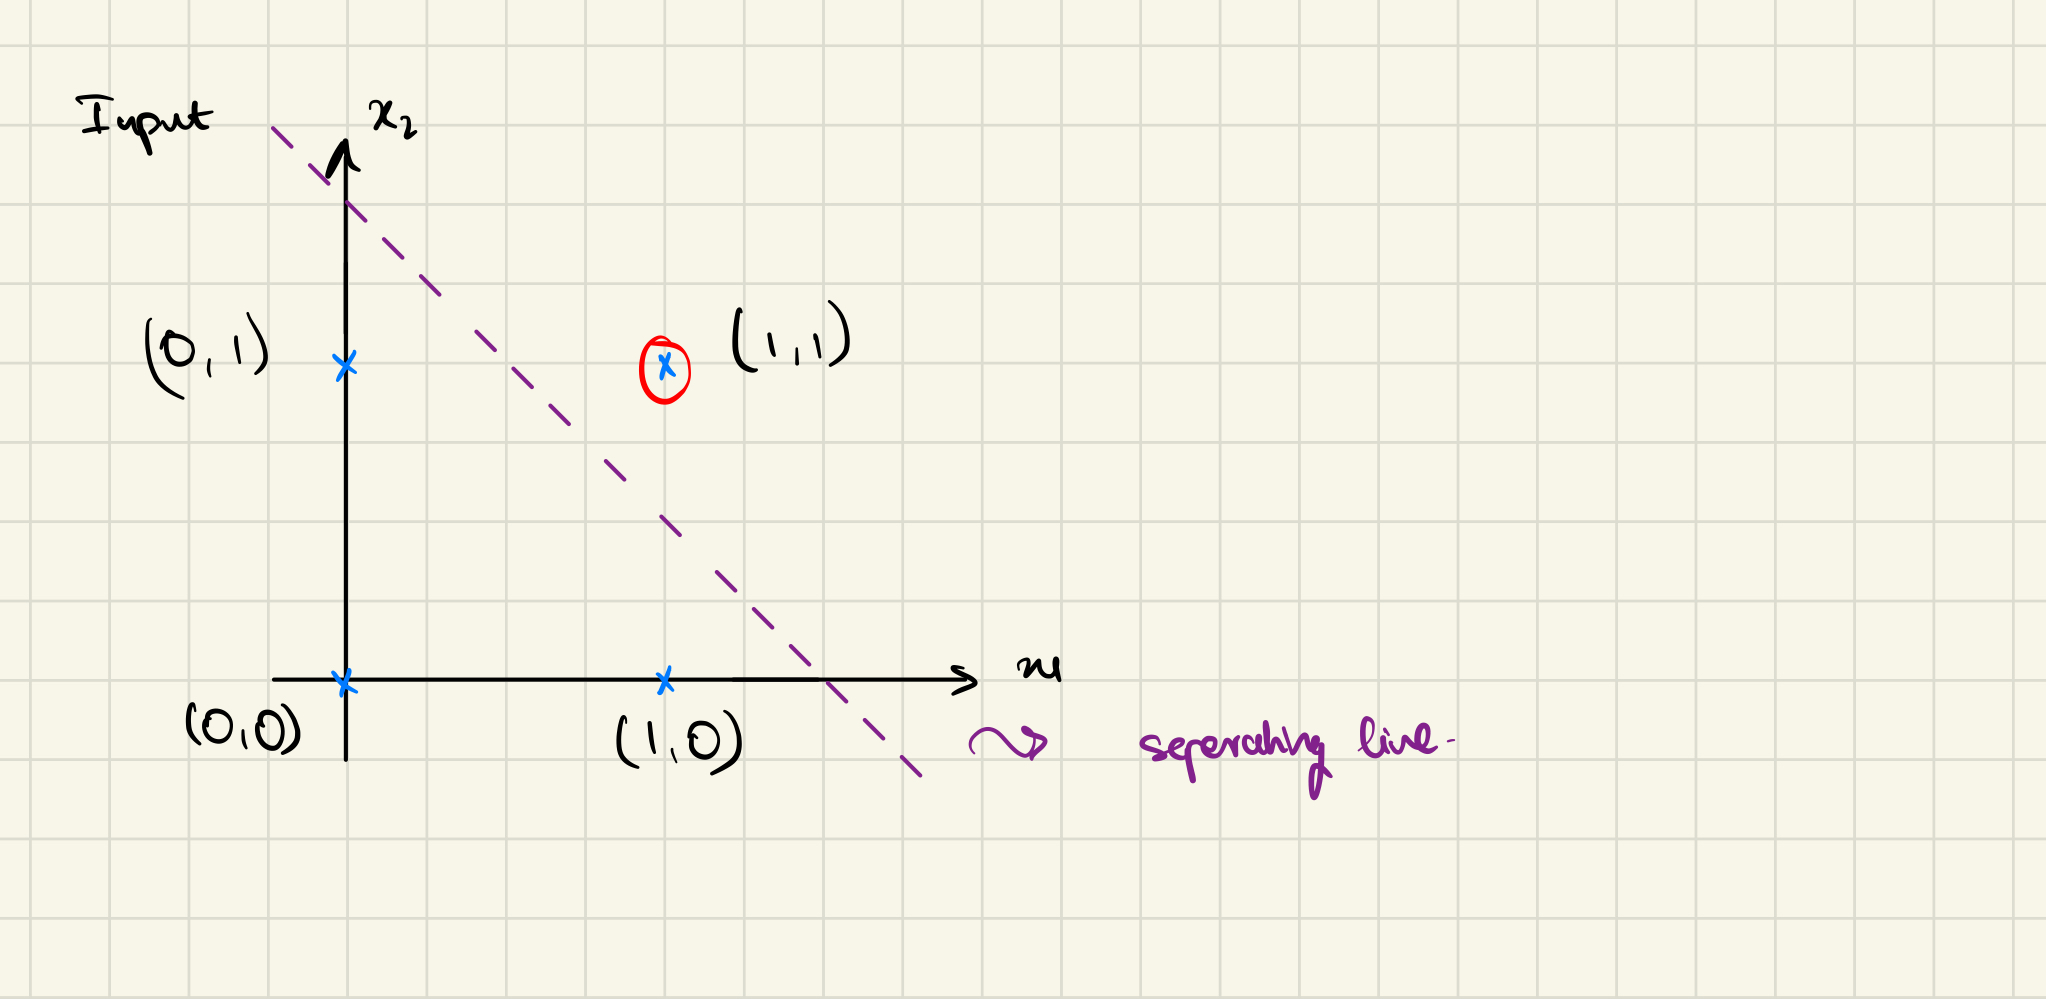
\includegraphics[scale=0.15]{CHAPTER_2/c2_fig_AND_function.jpeg}
  \caption{AND Function with separating line}
  \label{AND_function_2}
\end{figure}\\
The equation of the separating line in figure \ref{AND_function_2} is given by
\begin{align}
  x_1 + x_2 -1.5 = 0
\end{align}
We can transform the separating line in the form of $\textbf{w}^T\textbf{x} = 0$ to fit the perceptron.\\
Let 
\begin{align}
  \begin{matrix}
    \textbf{w} = \begin{bmatrix}
      -1.5 \\
      1 \\
      1
    \end{bmatrix} & \text{and} & \textbf{x} = \begin{bmatrix}
      1 \\
      x_1 \\
      x_2
    \end{bmatrix}
  \end{matrix}
\end{align}
Applying function (\ref{eq:mcp_neuron}) on each point to check whether they are correctly classified.
\begin{align}
  \nonumber
  \begin{matrix}
    \phi(p_1) = \phi\begin{pmatrix}
      \begin{bmatrix}
        -1.5 \\
        1 \\
        1 
      \end{bmatrix}.\begin{bmatrix}
        1 \\
        0 \\
        0
      \end{bmatrix}
    \end{pmatrix} = \phi(-1.5) = 0 
  \end{matrix}
\end{align}
\begin{align}
  \nonumber
  \begin{matrix}
    \phi(p_2) = \phi\begin{pmatrix}
      \begin{bmatrix}
        -1.5 \\
        1 \\
        1 
      \end{bmatrix}.\begin{bmatrix}
        1 \\
        1 \\
        0
      \end{bmatrix}
    \end{pmatrix} = \phi(-0.5) = 0
  \end{matrix}
\end{align}
\begin{align}
  \nonumber
  \begin{matrix}
    \phi(p_3) = \phi\begin{pmatrix}
      \begin{bmatrix}
        -1.5 \\
        1 \\
        1 
      \end{bmatrix}.\begin{bmatrix}
        1 \\
        1 \\
        1
      \end{bmatrix}
    \end{pmatrix} = \phi(0.5) = 1
  \end{matrix}
\end{align}
\begin{align}
  \nonumber
  \begin{matrix}
    \phi(p_4) = \phi\begin{pmatrix}
      \begin{bmatrix}
        -1.5 \\
        1 \\
        1 
      \end{bmatrix}.\begin{bmatrix}
        1 \\
        0 \\
        1
      \end{bmatrix}
    \end{pmatrix} = \phi(-0.5) = 0
  \end{matrix}
\end{align}
Thus, the perceptron is able to solve the AND function.
\subsection{OR Function}
The OR function returns a value of 1 if either of the inputs is 1. Let $f$ be the OR function such that
\begin{align}
\begin{matrix}
  \nonumber
  f(\textbf{p}_1) = 0 & f(\textbf{p}_2) = 1 & f(\textbf{p}_3) = 1 & f(\textbf{p}_4) = 1
\end{matrix}  
\end{align}
Consider the OR function with the separating line below
\begin{figure}[ht]
  \centering
  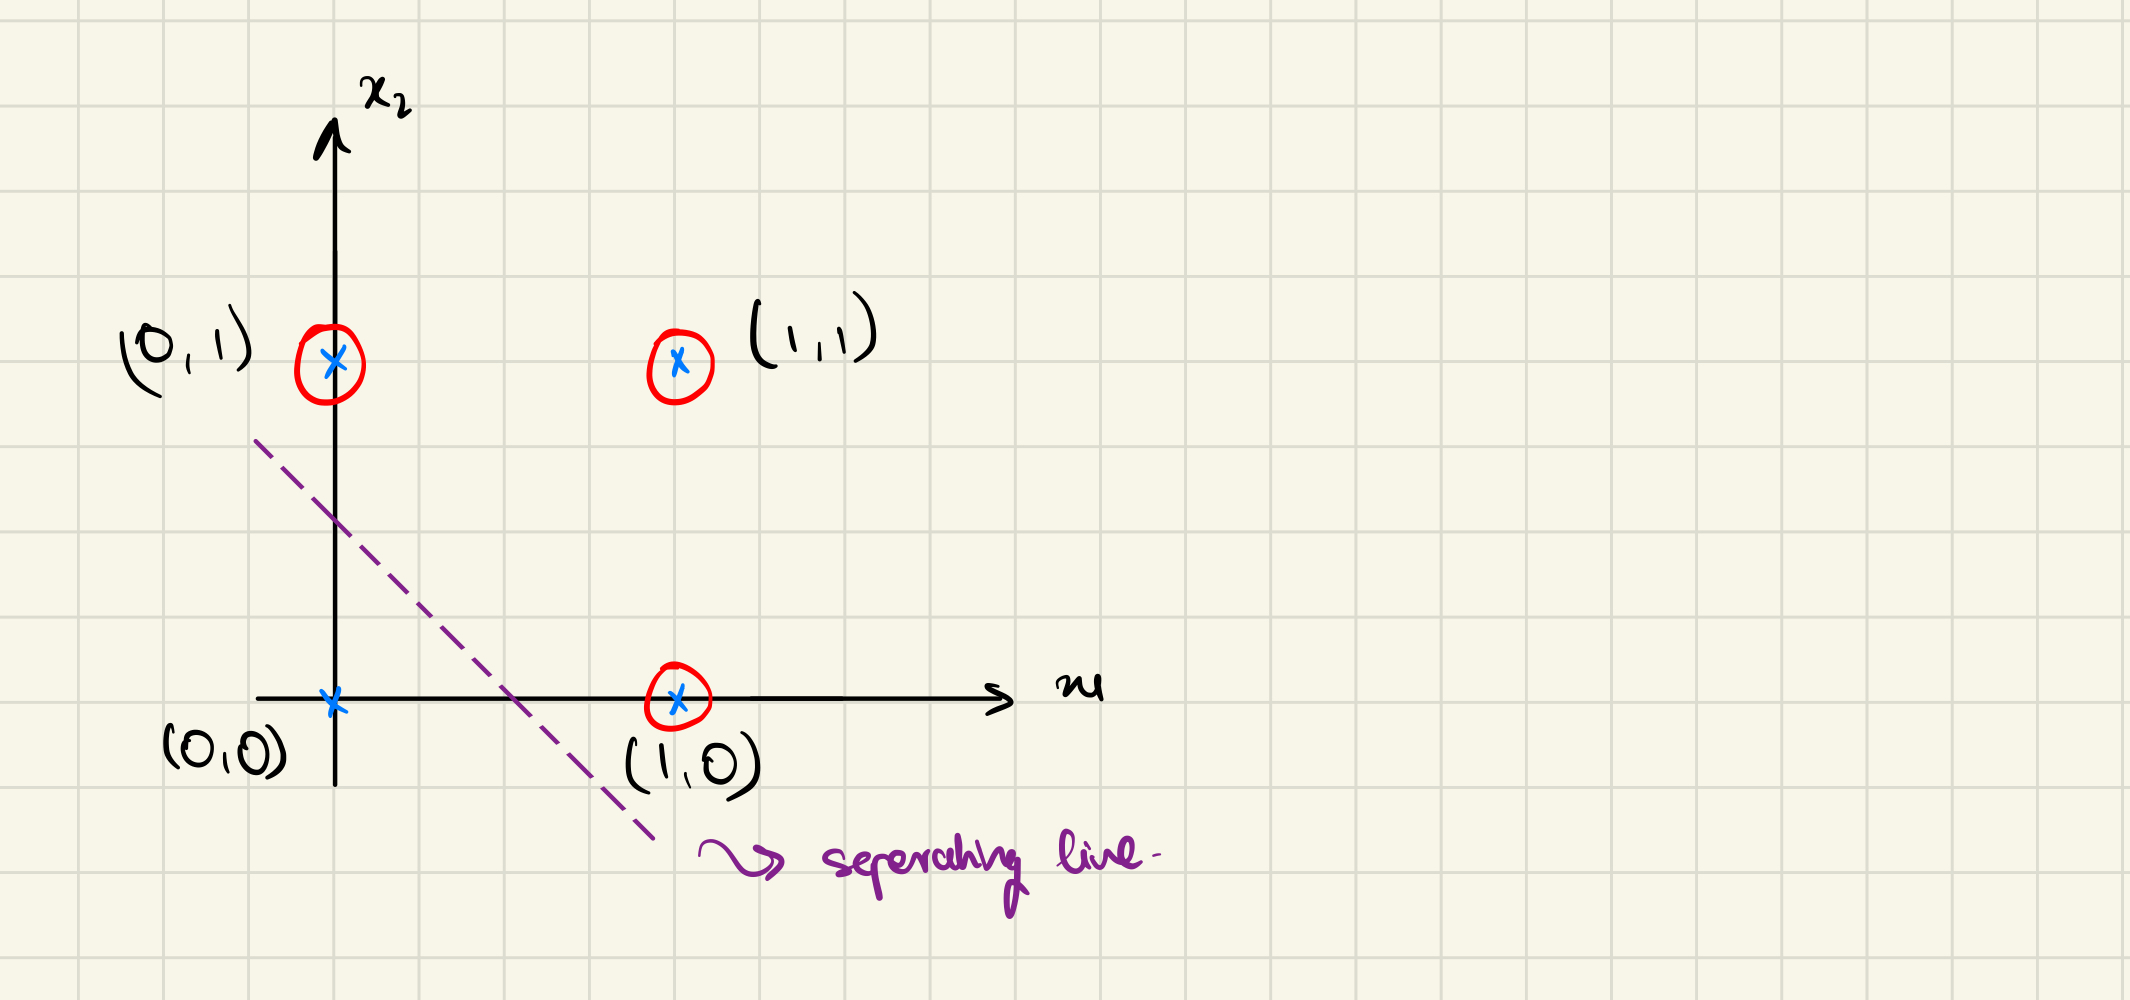
\includegraphics[scale=0.15]{CHAPTER_2/c2_fig_OR_function.jpeg}
  \caption{AND Function with separating line}
  \label{OR_function}
\end{figure}\\
The equation of the separating line in figure \ref{OR_function} is given by
\begin{align}
  x_1 + x_2 - 0.5 = 0
\end{align}
We can transform the separating line in the form of $\textbf{w}^T\textbf{x} = 0$ to fit the perceptron.\\
Let 
\begin{align}
  \begin{matrix}
    \textbf{w} = \begin{bmatrix}
      -0.5 \\
      1 \\
      1
    \end{bmatrix} & \text{and} & \textbf{x} = \begin{bmatrix}
      1 \\
      x_1 \\
      x_2
    \end{bmatrix}
  \end{matrix}
\end{align}
Applying function (\ref{eq:mcp_neuron}) on each point to check whether they are correctly classified.
\begin{align}
  \nonumber
  \begin{matrix}
    \phi(p_1) = \phi\begin{pmatrix}
      \begin{bmatrix}
        -0.5 \\
        1 \\
        1 
      \end{bmatrix}.\begin{bmatrix}
        1 \\
        0 \\
        0
      \end{bmatrix}
    \end{pmatrix} = \phi(-0.5) = 0 
  \end{matrix}
\end{align}
\begin{align}
  \nonumber
  \begin{matrix}
    \phi(p_2) = \phi\begin{pmatrix}
      \begin{bmatrix}
        -0.5 \\
        1 \\
        1 
      \end{bmatrix}.\begin{bmatrix}
        1 \\
        1 \\
        0
      \end{bmatrix}
    \end{pmatrix} = \phi(0.5) = 1
  \end{matrix}
\end{align}
\begin{align}
  \nonumber
  \begin{matrix}
    \phi(p_3) = \phi\begin{pmatrix}
      \begin{bmatrix}
        -0.5 \\
        1 \\
        1 
      \end{bmatrix}.\begin{bmatrix}
        1 \\
        1 \\
        1
      \end{bmatrix}
    \end{pmatrix} = \phi(1.5) = 1
  \end{matrix}
\end{align}
\begin{align}
  \nonumber
  \begin{matrix}
    \phi(p_4) = \phi\begin{pmatrix}
      \begin{bmatrix}
        -0.5 \\
        1 \\
        1 
      \end{bmatrix}.\begin{bmatrix}
        1 \\
        0 \\
        1
      \end{bmatrix}
    \end{pmatrix} = \phi(0.5) = 1
  \end{matrix}
\end{align}
Thus, the perceptron is able to solve the OR function.
\subsection{XOR Function}
The XOR function returns a value of 1 if either of the inputs is 1 but not both. Let $f$ be the XOR function such that
\begin{align}
  \begin{matrix}
    f(\textbf{p}_1)=0,&   f(\textbf{p}_2)=1 ,& f(\textbf{p}_3)=0,&   f(\textbf{p}_4)=1
    \label{eq:XOR_function}    
  \end{matrix}
\end{align}
Consider a plot of the XOR function below 
\begin{figure}[ht]
  \centering
  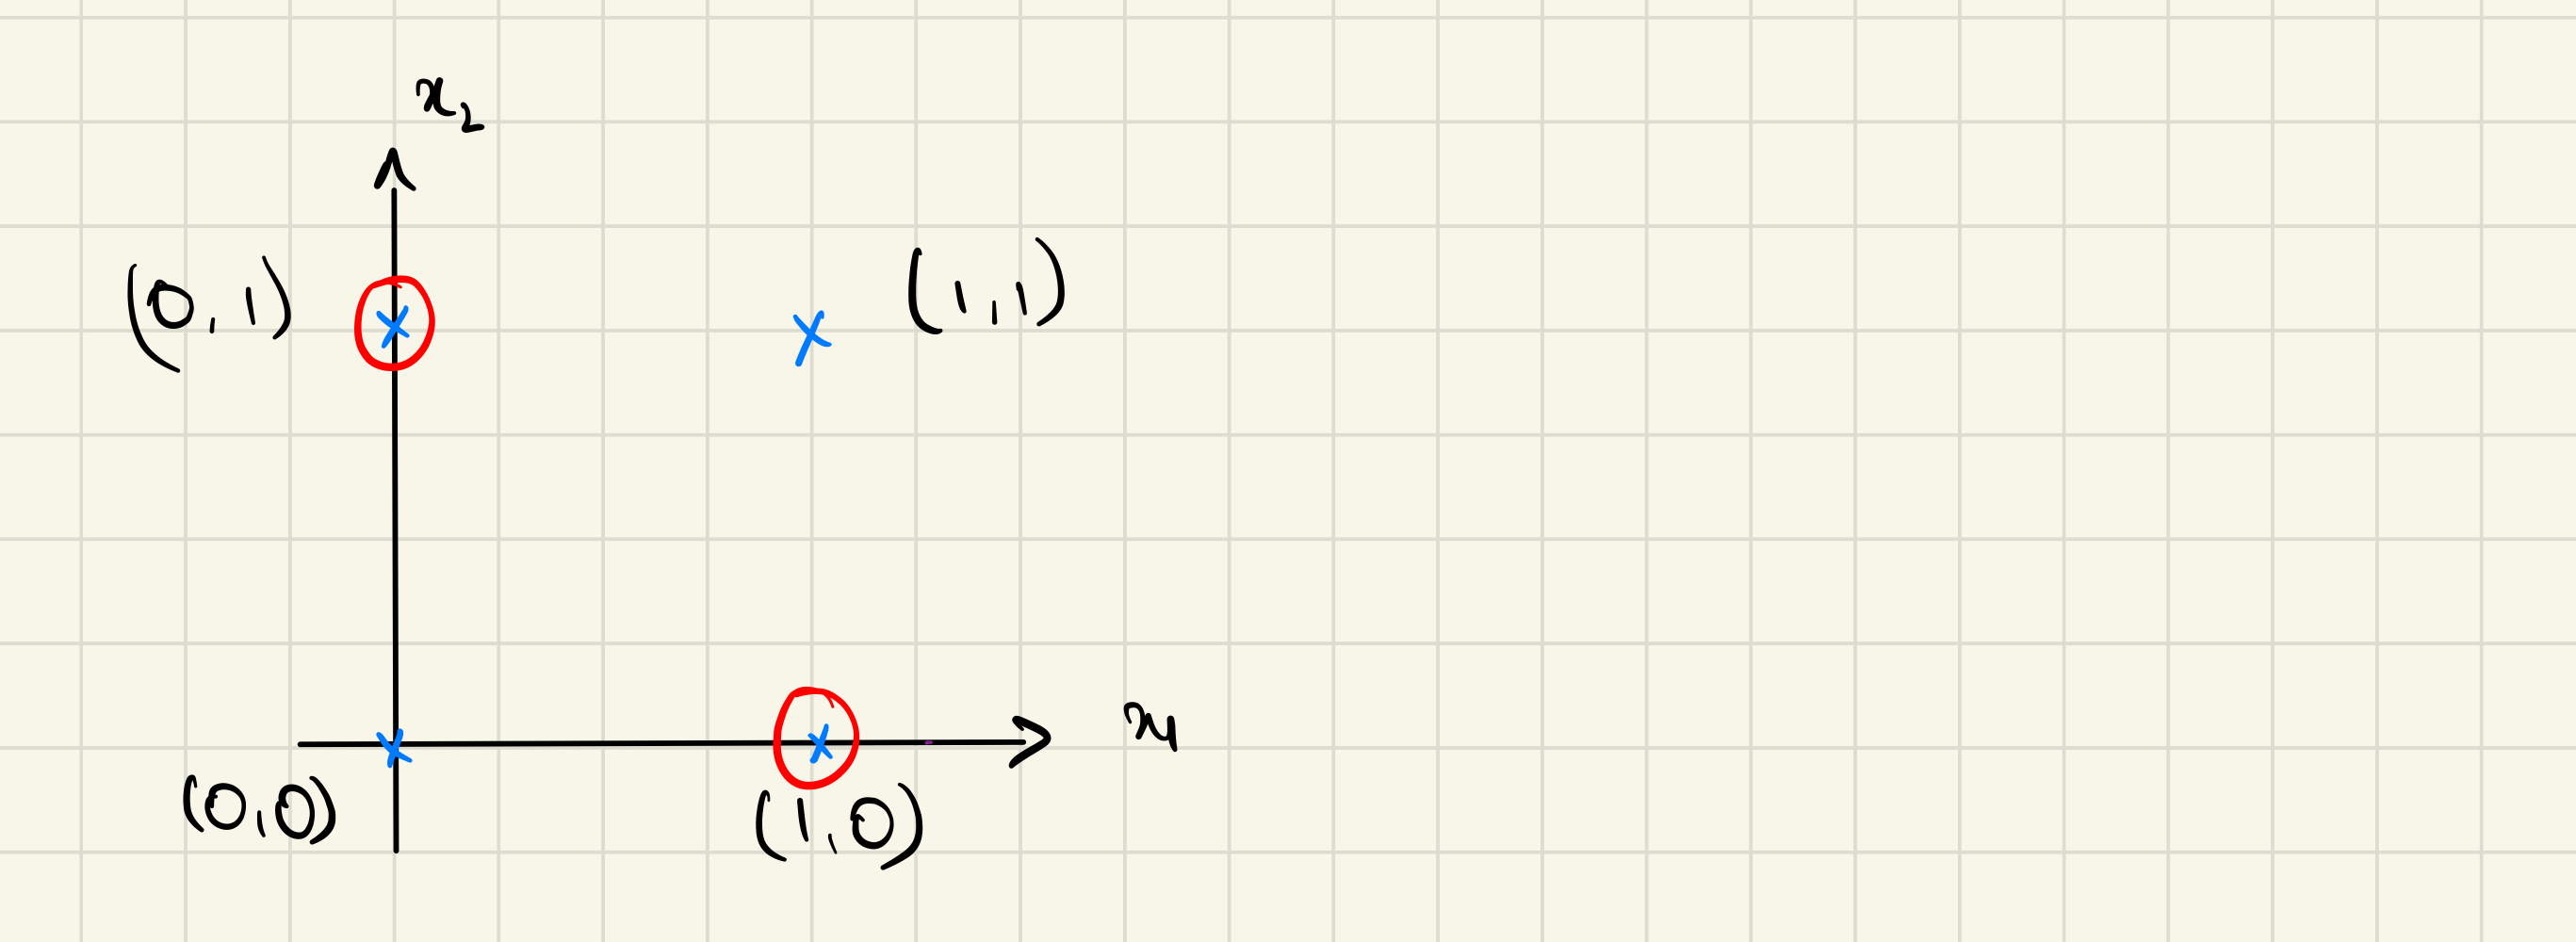
\includegraphics[scale=0.15]{CHAPTER_2/c2_rig_XOR.jpeg}
  \caption{OR function}
  \label{XOR_function}
\end{figure}\\
From figure \ref{XOR_function}; we can observe that no separating line alone could group the two different classes together. We attempt to find a combination of weight for the perceptron which reduces the error (margin) as much as possible.\\
\noindent Let $f^{*}$ be the exact function and $f(\textbf{x},\textbf{w}) = \textbf{w}^T\textbf{x} + b$, where $\textbf{w} = [w_1 \, \, w_2]^T$, be the approximate function. Consider the error function (the difference between the exact and approximate value)
\begin{align}
  \label{eq:error_XOR_prob}
  \mathbb{E}(\textbf{w},b) = \dfrac{1}{4} \sum_{x\in D}(f^{*}(\textbf{x})- \textbf{w}^T\textbf{x}-b)^2
\end{align}
we minimise the error function $\mathbb{E}$ by setting the partial derivatives to 0. The partial derivative with respect to the bias is given by
\begin{align}
  \nonumber
  \dfrac{\partial \mathbb{E}}{\partial b} &= -\dfrac{1}{2} \sum_{x\in D}(f^{*}(\textbf{x})- \textbf{w}^T\textbf{x}-b)\\
  \label{eq:bias_derivative}
  \dfrac{\partial \mathbb{E}}{\partial b} = 0\rightarrow \sum_{x\in D}f^{*}(\textbf{x}) &= \sum_{x\in D}\textbf{w}^T\textbf{x}- \sum_{x\in D}b
\end{align}
The partial derivative with respect to the weight vector is given by
\begin{align}
  \nonumber
  \dfrac{\partial \mathbb{E}}{\partial \textbf{x}} &= \dfrac{1}{2} \sum_{x\in D}(f^{*}(\textbf{x})- \textbf{w}^T\textbf{x}-b) \dfrac{\partial (-\textbf{w}^T\textbf{x})}{\partial \textbf{w}}\\
  \nonumber
  &=-\dfrac{1}{2} \sum_{x\in D}(f^{*}(\textbf{x})- \textbf{w}^T\textbf{x}-b)\textbf{x}\\
  \label{eq:weight_derivative}
  \dfrac{\partial \mathbb{E}}{\partial \textbf{w}} = 0\rightarrow \sum_{x\in D}\textbf{x}f^{*}(\textbf{x}) &= \sum_{x\in D}(\textbf{w}^T\textbf{x})\textbf{x} + b\sum_{x\in D}\textbf{x}
\end{align}
Substituting for values in equation (\ref{eq:bias_derivative})
\begin{align}
  \sum_{x\in D}f^{*}(\textbf{x}) &= f^{*}(\textbf{p}_1) + f^{*}(\textbf{p}_2) + f^{*}(\textbf{p}_3) + f^{*}(\textbf{p}_4) \nonumber \\
  &= 0+1+1+0 \nonumber \\
  & = 2 \\
  \sum_{x\in D}\textbf{w}^T\textbf{x} &= \textbf{w}^T\begin{bmatrix}
    0 \\
    0
  \end{bmatrix} + \textbf{w}^T\begin{bmatrix}
    1 \\
    0
  \end{bmatrix} + \textbf{w}^T\begin{bmatrix}
    1 \\
    1
  \end{bmatrix}+ \textbf{w}^T\begin{bmatrix}
    0 \\
    1
  \end{bmatrix} \nonumber \\
  &= 2w_1 + 2w_2 \\
  \nonumber
  \sum_{x\in D}b &= b \sum_{x\in D} 1 \\&= 4b
\end{align}
Thus, we get
\begin{align}
\nonumber 2 &= 2w_1 + 2w_2 + 4b \\
w_1 + w_2 + 2b &= 1
\label{eq:first_set_normal_eq}
\end{align}
Substituting for values in equation (\ref{eq:weight_derivative})
\begin{align}
  \sum_{x\in D}\textbf{x}f^{*}(\textbf{x}) &= \begin{bmatrix}
    0 \\
    0
  \end{bmatrix}(0) + \begin{bmatrix}
    1 \\
    0
  \end{bmatrix}(1) + \begin{bmatrix}
    1 \\
    1
  \end{bmatrix}(0)+ \begin{bmatrix}
    0 \\
    1
  \end{bmatrix}(1) \nonumber \\
  &= \begin{bmatrix}
    1 \\
    1
  \end{bmatrix}\\
  \nonumber
  \sum_{x\in D}(\textbf{w}^T\textbf{x})\textbf{x} &= \begin{bmatrix}
    w_1 & w_2
  \end{bmatrix} \begin{bmatrix}
    0 \\
    0
  \end{bmatrix} \begin{bmatrix}
    0 \\
    0
  \end{bmatrix} + \begin{bmatrix}
    w_1 & w_2
  \end{bmatrix} \begin{bmatrix}
    1 \\
    0
  \end{bmatrix} \begin{bmatrix}
    1 \\
    0
  \end{bmatrix} \\ \nonumber
  &+ \begin{bmatrix}
    w_1 & w_2
  \end{bmatrix} \begin{bmatrix}
    1 \\
    1
  \end{bmatrix} \begin{bmatrix}
    1 \\
    1
  \end{bmatrix} + \begin{bmatrix}
    w_1 & w_2
  \end{bmatrix} \begin{bmatrix}
    0 \\
    1
  \end{bmatrix} \begin{bmatrix}
    0 \\
    1
  \end{bmatrix} \\
  &= \begin{bmatrix}
    2w_1 + w_2 \\
    w_1 + 2w_2
  \end{bmatrix} \\
  \nonumber 
  b\sum_{x\in D}\textbf{x} &= 
    b\begin{bmatrix}
      0 \\
      0
    \end{bmatrix} + b\begin{bmatrix}
      1 \\
      0
    \end{bmatrix} + b\begin{bmatrix}
      1 \\
      1
    \end{bmatrix} + b\begin{bmatrix}
      0 \\
      1
    \end{bmatrix}\\
  &= b\begin{bmatrix}
    2 \\
    2
  \end{bmatrix}
\end{align}
Thus, we get
\begin{align}
  \label{eq:second_set_normal_eq}
\begin{bmatrix}
  1 \\
  1
\end{bmatrix}  &= \begin{bmatrix}
  2w_1 + w_2 \\
  w_1 + 2w_2
\end{bmatrix} + b\begin{bmatrix}
  2 \\
  2
\end{bmatrix}
\end{align}
From equations (\ref{eq:first_set_normal_eq}) and (\ref{eq:second_set_normal_eq}), we get the set of equations that forms the approximate function with the minimum error
\begin{align}
  w_1 + w_2 + 2b &= 1 \nonumber \\
  2w_1 + w_2 + 2b &= 1 \nonumber\\
  w_1 + 2w_2 + 2b &= 1 \nonumber
\end{align}
Solving the system of linear equations we get
\begin{align}
\begin{matrix}
  w_1 = 0 & w_2 = 0 & b = \dfrac{1}{2}
\end{matrix}  
\end{align}
Hence, the approximate function $f(\textbf{x},\textbf{w})$ is given by
\begin{align}
  f(\textbf{x},\textbf{w}) = \dfrac{1}{2}
\end{align}
\begin{figure}[ht]
  \centering
  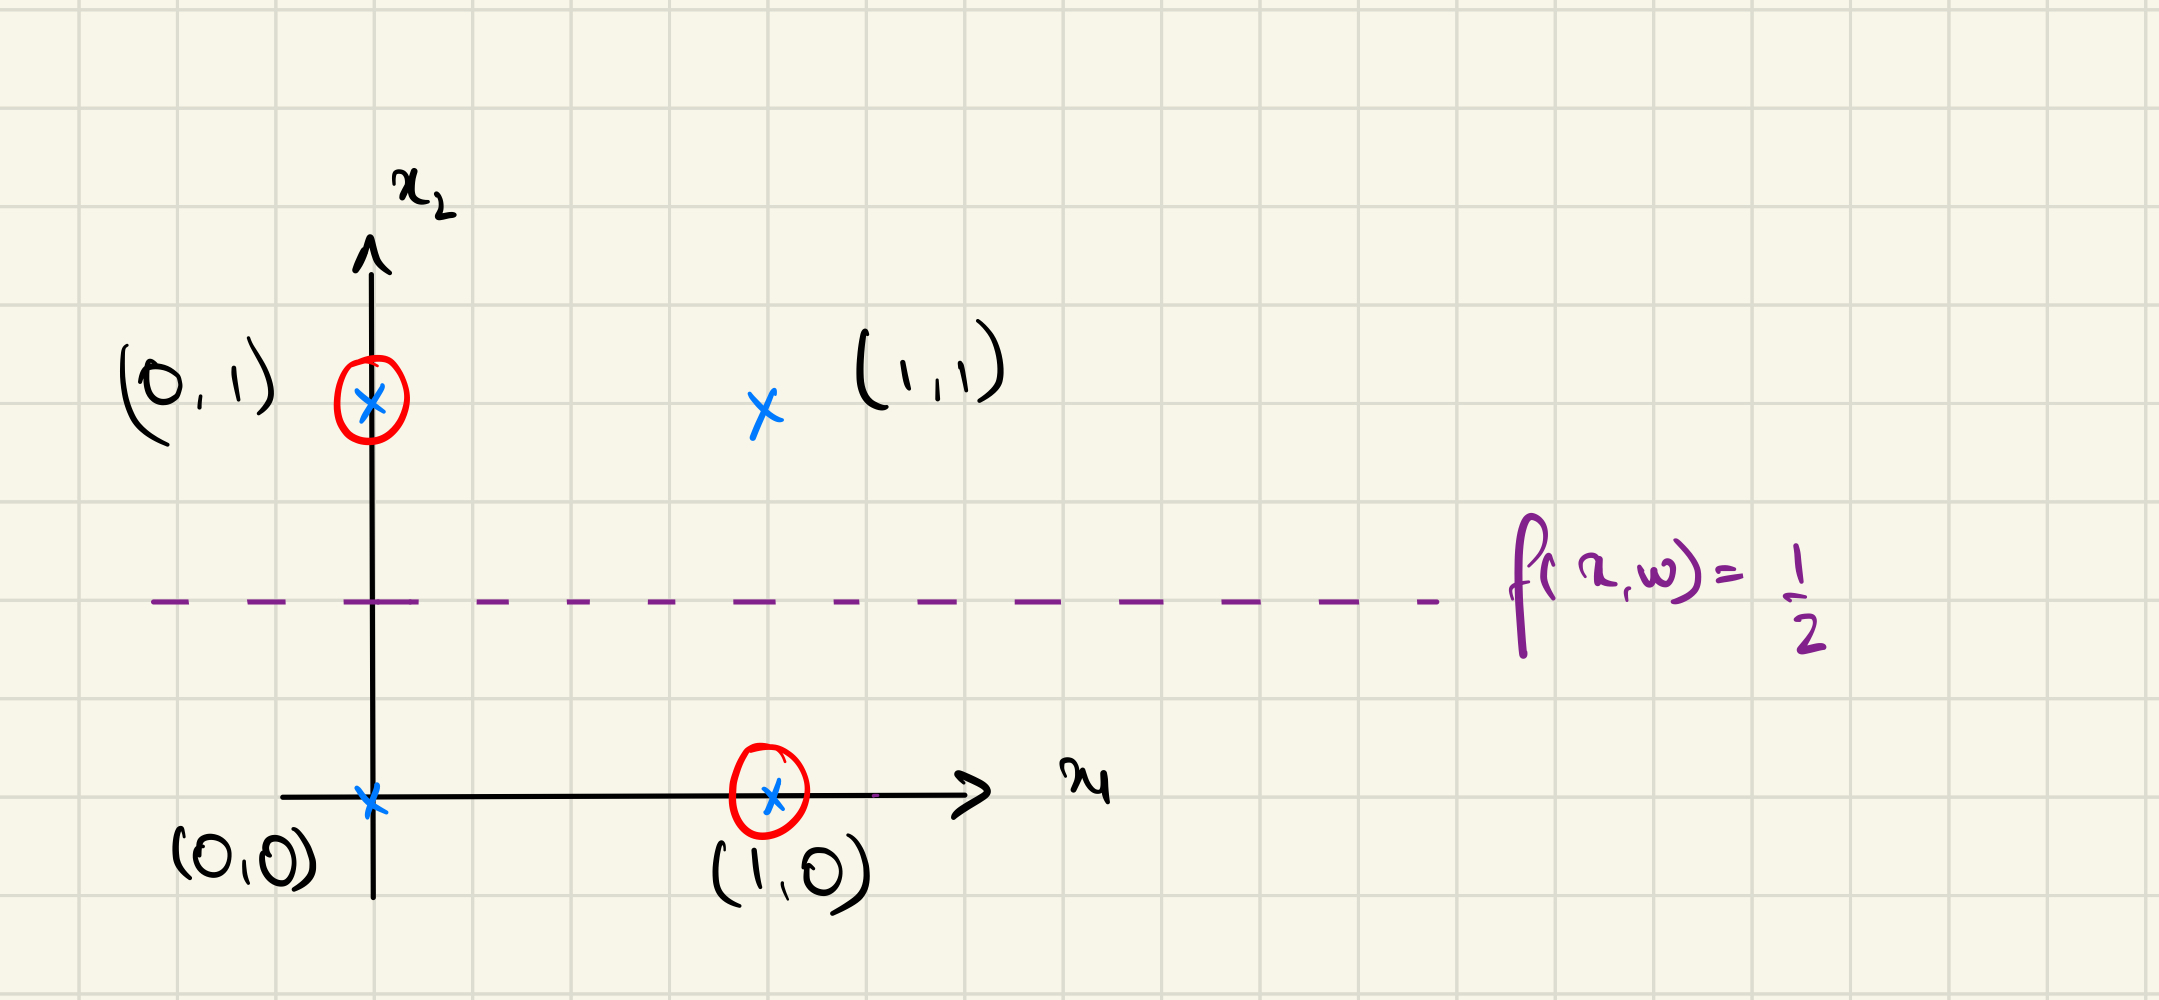
\includegraphics[scale=0.15]{CHAPTER_2/c2_fig_XOR_soln.jpeg}
  \caption{XOR approximate solution}
  \label{fig: approximate_XOR_solution}
\end{figure}\\
\noindent  Clearly from figure \ref{fig: approximate_XOR_solution}, the perceptron model cannot solve the XOR logic function. The XOR problem is actually not linearly separable. Thus, we introduce \textbf{feedforward networks} to overcome this problem.
\section{Feedforward Network}
We have seen that the single perceptron cannot solve the XOR problem. In order to solve the problem, we use a set of perceptrons that learns two different functions within a connected network.\vspace{5mm} \\
First, let's consider two NOT boolean function $f_1^{*} = x_1 \text{ AND } (\text{NOT }x_2)$ and $f_2^{*} = (\text{NOT }x_1) \text{ AND } x_2$. \vspace{5mm}\\
Consider $f_1^{*}$ which returns 1 if $x_1$ and (not $x_2$) are equal to 1.
\begin{table}
  \begin{center}
    \begin{tabular}{ c c c c}
      $x_1$ & $x_2$ & NOT ($x_2$) & $x_1$ AND (NOT $x_2$) \\
     \hline 
      0 & 0 & 1 & 0 \\  
      1 & 0 & 1 & 1 \\  
      1 & 1 & 0 & 0 \\  
      0 & 1 & 0 & 0 
    \end{tabular}
    \caption{Truth Table for $f_1^{*}$}
  \label{table:truth_table_f_1}
  \end{center}  
\end{table} \vspace{5mm}\\
The function $f_1^{*}$ can be separated using the perceptron.
\begin{figure}[ht]
  \centering
  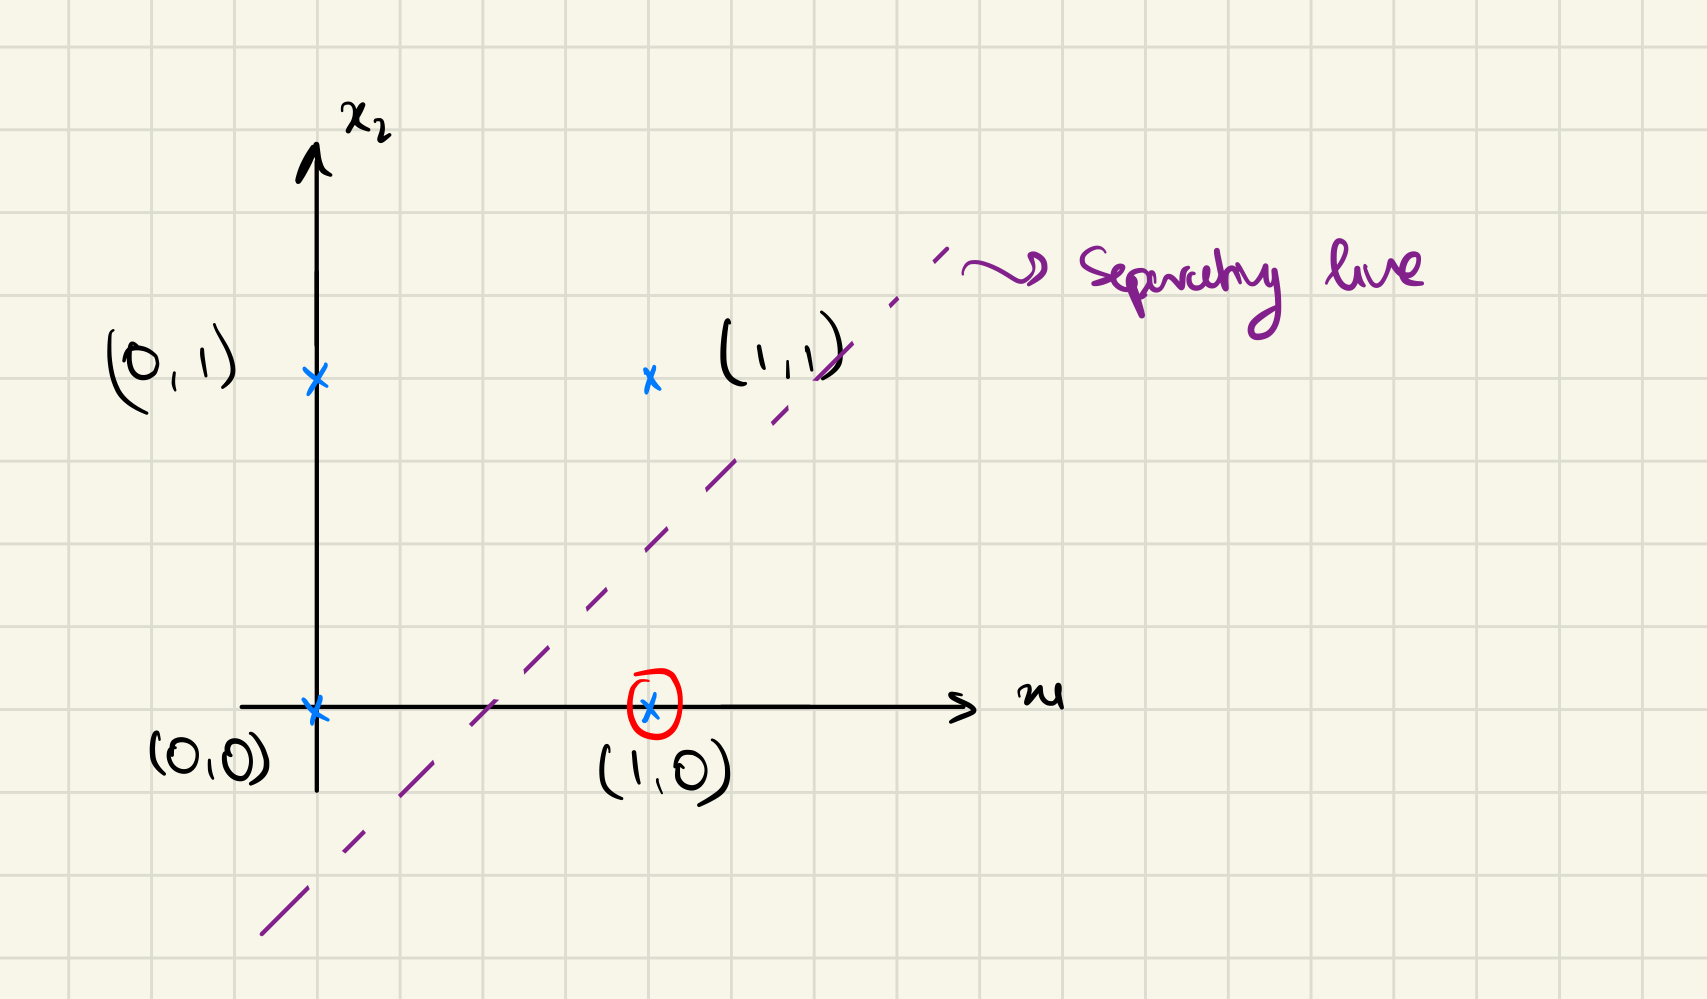
\includegraphics[scale=0.15]{CHAPTER_2/c2_fig_f_1_XOR.jpeg}
  \caption{$f_1$}
  \label{fig:f1_XOR}
\end{figure} \\
The equation of the separating line in figure \ref{fig:f1_XOR} is given by
\begin{align}
  x_1 - x_2 - \dfrac{1}{2} = 0
\end{align}
We can transform the separating line in the form of $\textbf{w}^T\textbf{x} = 0$ to fit the perceptron.
\begin{align}
  \label{eq: weight_f_1}
  \begin{matrix}
    \textbf{w} = \begin{bmatrix}
      -0.5 \\
      1 \\
      -1
    \end{bmatrix} & \text{and} & \textbf{x} = \begin{bmatrix}
      1 \\
      x_1 \\
      x_2
    \end{bmatrix}
  \end{matrix}
\end{align}
Similarly, consider $f_2^{*}$ which returns 1 if (not $x_1$) and $x_2$ are equal to 1.
\begin{table}
  \begin{center}
    \begin{tabular}{ c c c c}
      $x_1$ & $x_2$ & NOT ($x_1$) & (NOT $x_1$) AND $x_2$ \\
     \hline 
      0 & 0 & 1 & 0 \\  
      1 & 0 & 0 & 0 \\  
      1 & 1 & 0 & 0 \\  
      0 & 1 & 1 & 1 
    \end{tabular}
    \caption{Truth Table for $f_2^{*}$}
  \label{table:truth_table_f_2}
  \end{center}  
\end{table} \vspace{40mm}\\
The function $f_2^{*}$ can be separated using the perceptron.
\begin{figure}[ht]
  \centering
  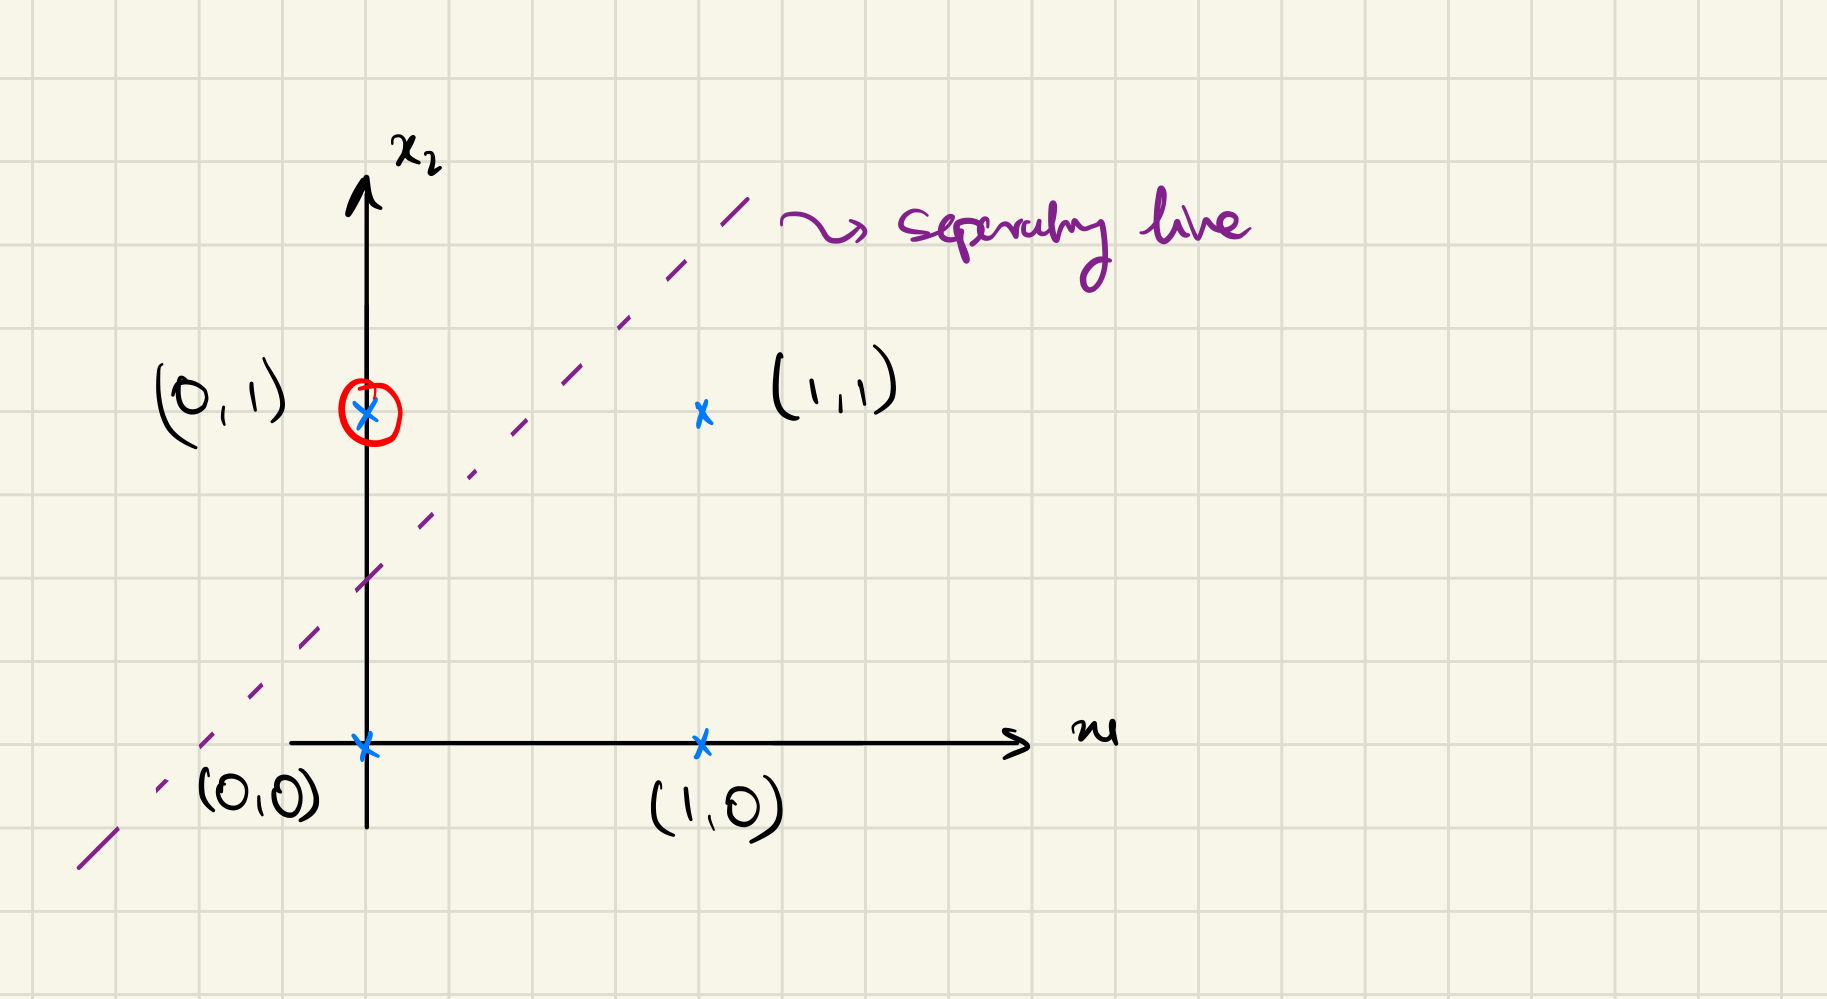
\includegraphics[scale=0.15]{CHAPTER_2/c2_fig_f_2_XOR.jpeg}
  \caption{$f_1$}
  \label{fig:f2_XOR}
\end{figure} \\
The equation of the separating line in figure \ref{fig:f2_XOR} is given by
\begin{align}
  -x_1 + x_2 - \dfrac{1}{2} = 0
\end{align}
We can transform the separating line in the form of $\textbf{w}^T\textbf{x} = 0$ to fit the perceptron.
\begin{align}
  \label{eq: weight_f_2}
  \begin{matrix}
    \textbf{w} = \begin{bmatrix}
      -0.5 \\
      -1 \\
      1
    \end{bmatrix} & \text{and} & \textbf{x} = \begin{bmatrix}
      1 \\
      x_1 \\
      x_2
    \end{bmatrix}
  \end{matrix}
\end{align}
Consequently, the XOR function defined in (\ref{eq:XOR_function}) can be expressed as $f^*$ such that
\begin{align}
  \nonumber
  f^*(x_1,x_2) = f_1^*(x_1,x_2) \text{ OR } f_2^*(x_1,x_2)
\end{align}
\begin{table}
  \begin{center}
    \begin{tabular}{ c c c c c}
      $x_1$ & $x_2$ & $f_1^*(x_1,x_2)$ & $f_2^*(x_1,x_2)$ &$f_2^*(x_1,x_2)$ \\
     \hline 
      0 & 0 & 0 & 0 & 0\\  
      1 & 0 & 1 & 0 & 1\\  
      1 & 1 & 0 & 0 & 0\\  
      0 & 1 & 0 & 1 & 1
    \end{tabular}
    \caption{Truth Table for $f^{*}$}
  \label{table:truth_table_f*}
  \end{center}  
\end{table}\vspace{20mm}\\
Consider a feedforward network with a hidden layer with two units $h_1$ and $h_2$ such that $h_1$ learns $f_1^*(x_1,x_2)$ and $h_2$ learns $f_2^*(x_1,x_2)$.
\begin{align}
  h_1 &= f_1^*(x_1,x_2) \nonumber\\
  &= \phi(z_1) \nonumber
\end{align}
where $z_1 = w_{11}x_1 + w_{12}x_2 + b_1$ and $w_{11} = 1$, $w_{12} = -1$ and $b_1=-0.5$ from separating line in (\ref{eq: weight_f_1}).
\begin{align}
  h_2 &= f_2^*(x_1,x_2) \nonumber\\
  &= \phi(z_2) \nonumber
\end{align}
where $z_2 = w_{21}x_1 + w_{22}x_2 + b_1$ and $w_{21} = -1$, $w_{22} = 1$ and $b_2 = -0.5$ from separating line in (\ref{eq: weight_f_2}).
\begin{figure}[ht]
  \centering
  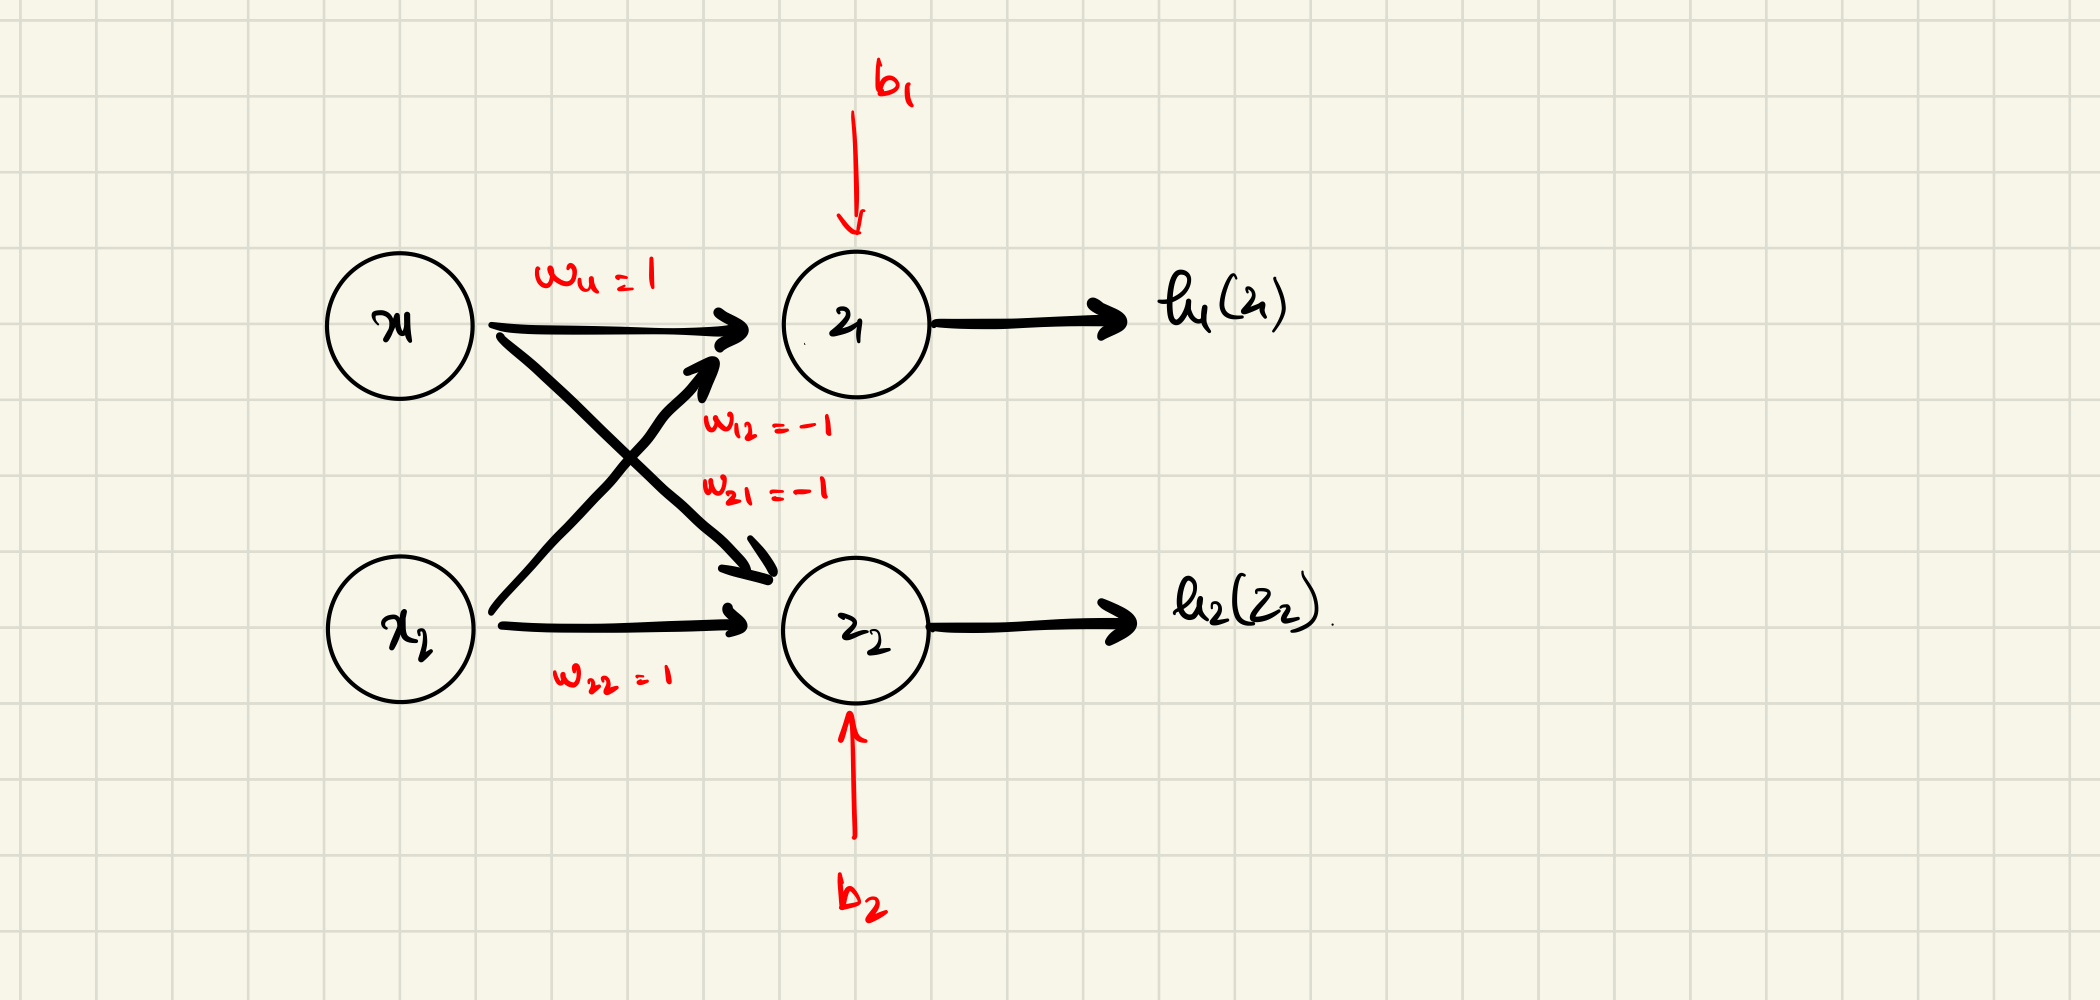
\includegraphics[scale=0.15]{CHAPTER_2/c2_fig_hidden_layer.jpeg}
  \caption{FFN hidden layer}
  \label{fig:hidden_layer_only}
\end{figure} \\
Thus we obtain the system below for the hidden layer.
\begin{align}
  \begin{bmatrix}
    z_1 \\
    z_2
  \end{bmatrix} = \begin{bmatrix}
    b_1 & w_{11} & w_{12}   \\
    b_1 & w_{21} & w_{22}
  \end{bmatrix} \begin{bmatrix}
    1\\
    x_1 \\
    x_2
  \end{bmatrix}
\end{align}
We then feed forward the information from the hidden layer to another layer.
\begin{align}
  \begin{bmatrix}
    h_1 \\
    h_2
  \end{bmatrix} = \phi\begin{pmatrix}
    \begin{bmatrix}
      z_1 \\
      z_2
    \end{bmatrix}
  \end{pmatrix}
\end{align}
At the hidden layer, we are left with the following truth table.\\
\begin{table}[ht]
  \begin{center}
    \begin{tabular}{ c c c c}
      $x_1$ & $x_2$ & XOR \\
     \hline 
      0 & 0 & 0 & \\  
      1 & 0 & 1 & \\  
      0 & 0 & 0 & \text{redundant}\\  
      0 & 1 & 1 & 
    \end{tabular}
    \caption{Truth Table from hidden layer}
  \label{table:truth_table_hidden_layer}
  \end{center}  
\end{table}\\
The XOR problem can not be separated from using another perceptron after the hidden layer.
\begin{figure}[ht]
  \centering
  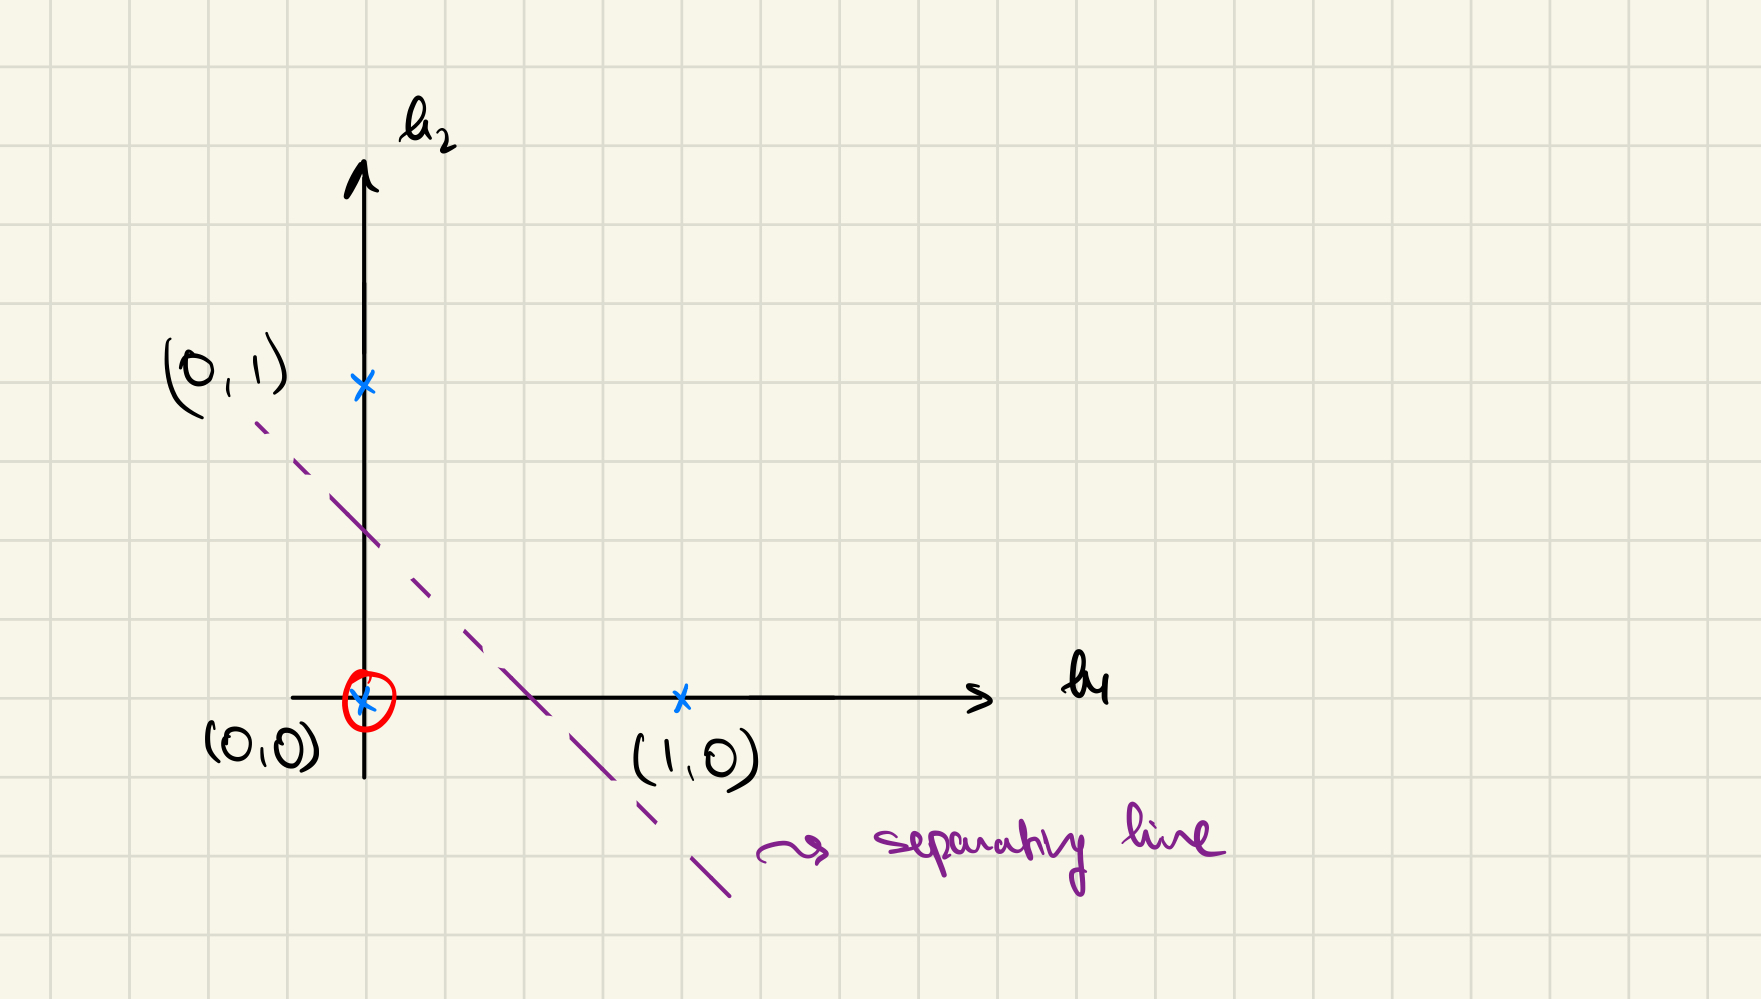
\includegraphics[scale=0.15]{CHAPTER_2/c2_fig_XOR_sep.jpeg}
  \caption{XOR layer}
  \label{fig:XOR layer}
\end{figure}\\
The equation of the separation line is in figure (\ref{fig:XOR layer}) is given binary
\begin{align}
h_1 + h_2 - \dfrac{1}{2} = 0  
\end{align}
We can now transform the separating line in the form of $\textbf{w}^T\textbf{x} = 0$ to fit the perceptron.
\begin{align}
  \begin{matrix}
    \textbf{w} = \begin{bmatrix}
      -0.5 \\
      1 \\
      1
    \end{bmatrix} & \textbf{h} = \begin{bmatrix}
      1 \\
      h_1 \\
      h_2
    \end{bmatrix}  
  \end{matrix}
\end{align}
Finally, the XOR function can be represented using the set of transform defined below.
\begin{align}
  \begin{matrix}
    f(x_1,x_2) = \phi^{'} \begin{pmatrix}
    \textbf{w}_2^T 
    \begin{pmatrix}
      \phi \begin{pmatrix}
        \textbf{w}_1^T\textbf{x}
    \end{pmatrix}  
  \end{pmatrix}
  \end{pmatrix}
\end{matrix}
\end{align}
where
\begin{align}
  \begin{matrix}
  \textbf{x} = \begin{bmatrix}
    1 \\
    x_1 \\
    x_2
  \end{bmatrix} & \textbf{w}_1 = \begin{bmatrix}
    -0.5 & -0.5 \\
    1 & -1  \\
    -1 & 1 
  \end{bmatrix} & \textbf{w}_2 = \begin{bmatrix}
    -0.5 \\
    1 \\
    1
  \end{bmatrix} 
  \end{matrix}
\end{align}
$\phi^{'}$ taken an augmented input from the calculation of $\phi(\textbf{w}_1^T \textbf{x})$ to accommodate for the bias.
\begin{figure}[ht]
  \centering
  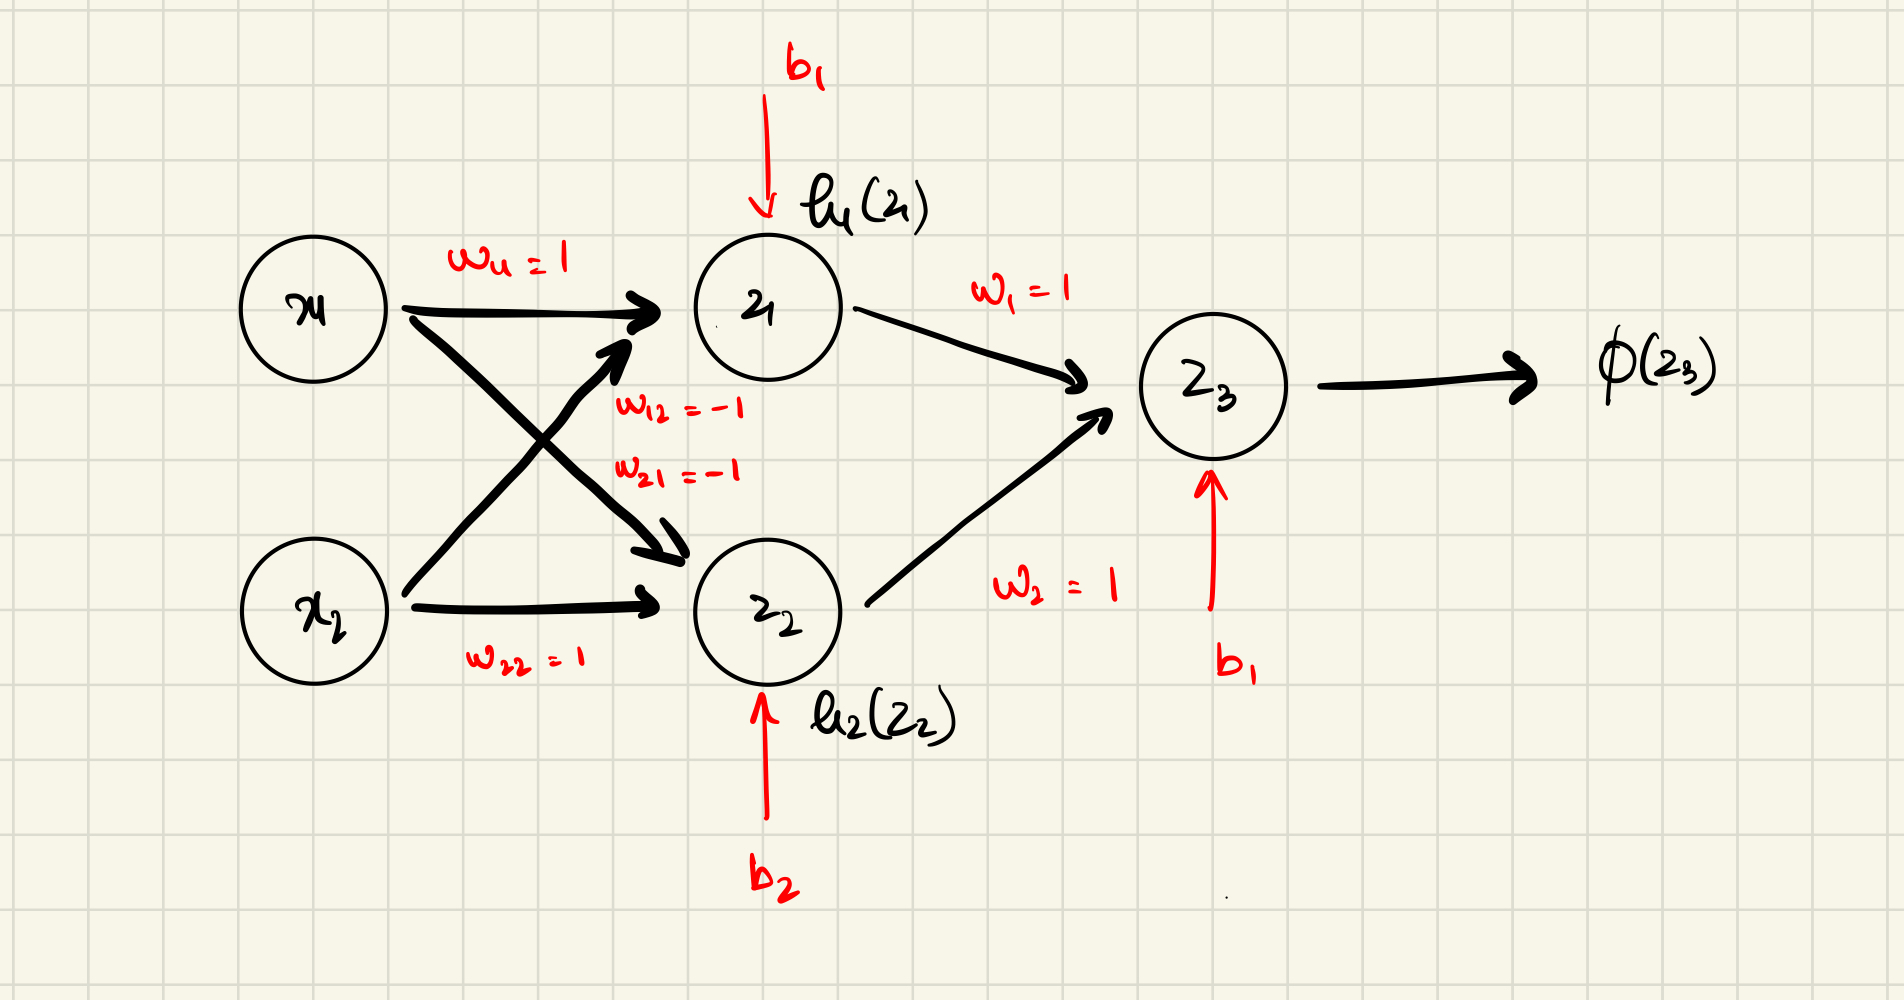
\includegraphics[scale=0.15]{CHAPTER_2/c2_fig_XOR_final.jpeg}
  \caption{Feedforward network for XOR problem}
  \label{fig: ffn_XOR_final}
\end{figure}\vspace{30mm}\\
\textbf{Checking for $\textbf{x} = \begin{bmatrix} 1 & 0 & 0 \end{bmatrix}^T$}
\begin{align*}
  \textbf{w}_1^T\textbf{x} &= \begin{bmatrix}
    -0.5 & 1 & -1 \\
    -0.5 & -1 & 1 
  \end{bmatrix} \begin{bmatrix}
    1\\
    0 \\
    0
  \end{bmatrix} = \begin{bmatrix}
    -0.5 \\
    -0.5
  \end{bmatrix} \\
  \phi(\textbf{w}_1^T\textbf{x}) &= \phi\begin{pmatrix}
    \begin{bmatrix}
      -0.5 \\
      -0.5
    \end{bmatrix}
  \end{pmatrix} = \begin{bmatrix}
    0 \\
    0
  \end{bmatrix} \\
  \phi^{'} \begin{pmatrix}
    \textbf{w}_2^T 
    \begin{pmatrix}
      \phi \begin{pmatrix}
        \textbf{w}_1^T\textbf{x}
    \end{pmatrix}  
  \end{pmatrix}
  \end{pmatrix} &= \phi^{'}\begin{pmatrix}
    \begin{bmatrix}
      -0.5 & 1 & 1
    \end{bmatrix} \begin{bmatrix}
      1 \\ 
      0 \\
      0
    \end{bmatrix}
  \end{pmatrix} = \phi^{'}(-0.5)
\end{align*}
Thus, for $\textbf{p}_1 = \begin{bmatrix}
  0,0
\end{bmatrix}^T$
\begin{align*}
  f(x_1,x_2) = \phi^{'} (-0.5) = 0
\end{align*}
\textbf{Checking for $\textbf{x} = \begin{bmatrix} 1 & 0 & 1 \end{bmatrix}^T$}
\begin{align*}
  \textbf{w}_1^T\textbf{x} &= \begin{bmatrix}
    -0.5 & 1 & -1 \\
    -0.5 & -1 & 1 
  \end{bmatrix} \begin{bmatrix}
    1\\
    0 \\
    1
  \end{bmatrix} = \begin{bmatrix}
    -1.5 \\
    0.5
  \end{bmatrix} \\
  \phi(\textbf{w}_1^T\textbf{x}) &= \phi\begin{pmatrix}
    \begin{bmatrix}
      -1.5 \\
      0.5
    \end{bmatrix}
  \end{pmatrix} = \begin{bmatrix}
    0 \\
    1
  \end{bmatrix} \\
  \phi^{'} \begin{pmatrix}
    \textbf{w}_2^T 
    \begin{pmatrix}
      \phi \begin{pmatrix}
        \textbf{w}_1^T\textbf{x}
    \end{pmatrix}  
  \end{pmatrix}
  \end{pmatrix} &= \phi^{'}\begin{pmatrix}
    \begin{bmatrix}
      -0.5 & 1 & 1
    \end{bmatrix} \begin{bmatrix}
      1 \\ 
      0 \\
      1
    \end{bmatrix}
  \end{pmatrix} = \phi^{'}(0.5)
\end{align*}
Thus, for $\textbf{p}_4 = \begin{bmatrix}
  0,0
\end{bmatrix}^T$
\begin{align*}
  f(x_1,x_2) = \phi^{'} (0.5) = 1
\end{align*}
\section{Backpropagation}